\chapter{Implementación}
En este séptimo capítulo se detallará la implementación del sistema. En primer lugar,  se presentará la estructura del proyecto que se ha realizado para el frontend y del backend y, a continuación,
se describirá la implementación de cada una de las funcionalidades del sistema, presentando la documentación de cada ruta de la API y describiendo el código escrito durante el desarrollo.

\section{Herramientas utilizadas}
En el desarrollo de la aplicación se utilizarán varias herramientas externas que ayudarán en el cumplimiento de los objetivos y facilitarán la implementación de cada una de las historias de usuario. A continuación se muestran algunas
de ellas:

\subsection{Git \& Github}
Git es una herramienta para el control de versiones. Nos permitirá mantener un historial de cambios que nos ayudarán en la implementación cuando necesitemos "volver atrás", así como poder trabajar en distintas ramas cuando la situación lo requiera (por ejemplo, si encontramos un error puedo abrir una nueva rama para poder trabajar exclusivamente en arreglarlo).

Como complemento a Git, usaremos Github, una plataforma para alojar repositorios de Git. En Github tendremos un repositorio para el frontend y para el backend, donde se irán subiendo los cambios que se vayan realizando. Esto facilitará la posibilidad de trabajar en el desarrollo en varios dispositivos permitiendo un desarrollo más flexible en cuanto a en qué dispositivo y cuándo trabajar. 

\subsection{Jira}
Jira es una herramienta para la gestión de proyectos. Usaré Jira para facilitar el cumplimiento de algunos de los principios de metodologías ágiles que usamos en la planificación y controlar el seguimiento de esta última. En Jira tendré un Sprint Backlog, cuyas historias de usuario y tareas irán moviéndose a los distintos Sprints para su desarrollo.

\begin{figure}[H]
  \centering
  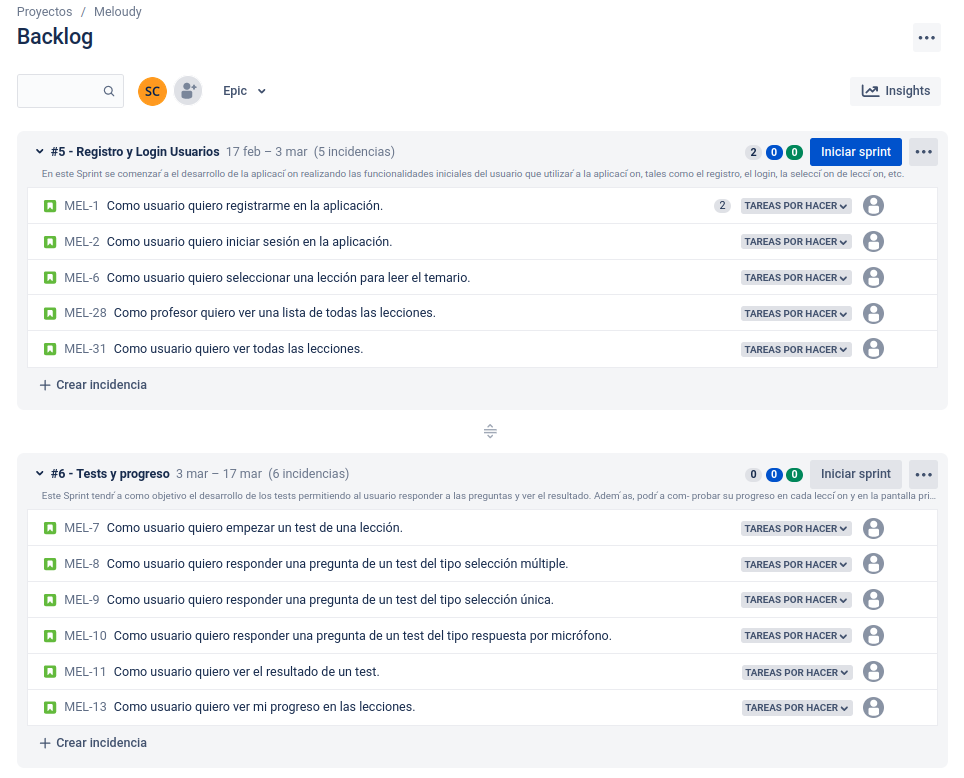
\includegraphics[width=\textwidth]{imagenes/c7/jira.png}
  \caption{Captura de pantalla de Jira. En ella se puede ver el Sprint Backlog, donde se encuentran las historias de usuario repartidas entre los sprints.}
  \label{fig:login}
\end{figure}


\subsection{Visual Studio Code \& Android Studio}
Visual Studio Code es el editor de código fuente que se usará para implementar la parte backend (NodeJS) de nuestro sistema. Nos permitirá un desarrollo más cómodo y eficiente, ya que nos ofrece una gran variedad de herramientas para el desarrollo, como la posibilidad de depurar el código, herramientas para el formato de los distintos lenguajes de programación, visualizador de versiones de Git, etc.

Android Studio es el entorno de desarrollo integrado oficial para la plataforma Android. Se utilizará para implementar la parte de frontend (flutter) y para ejecutar la aplicación en un simulador de Android o en nuestro propio dispositivo físico.

\subsection{Mongo Compass}
Mongo Compass es una herramienta interactiva para la consulta, la gestión y el análisis de los datos en MongoDB. Se utilizará para comprobar si las consultas se realizan correctamente y para añadir datos a la base de datos (lecciones, preguntas...) de forma fácil, cómoda y rápida.

\begin{figure}[H]
  \centering
  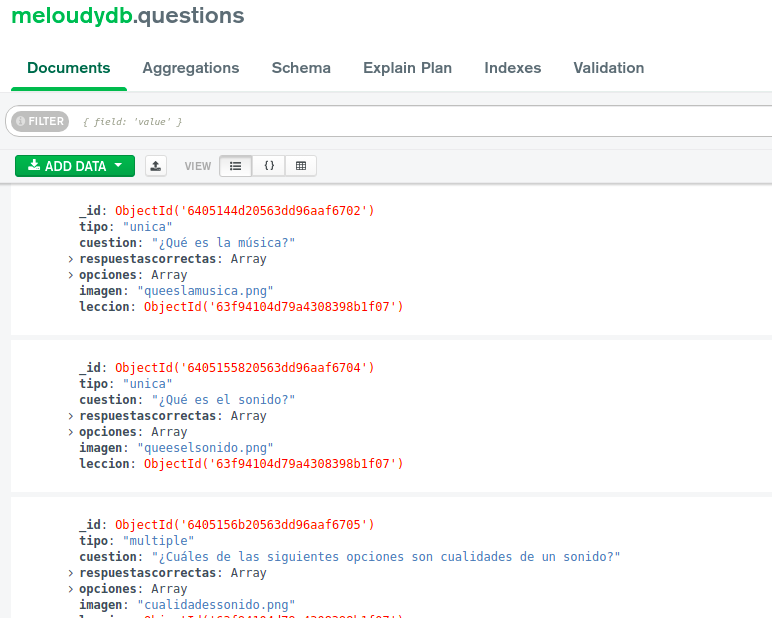
\includegraphics[width=\textwidth]{imagenes/c7/compass.png}
  \caption{Captura de pantalla de Jira. En ella se puede ver el Sprint Backlog, donde se encuentran las historias de usuario repartidas entre los sprints.}
  \label{fig:login}
\end{figure}

\subsection{Postman}
Postman es una plataforma API para diseñar, construir, probar e iterar APIs. Se utilizará en la implementación de nuestra aplicación para comprobar el funcionamiento de las rutas especificadas y codificadas en el backend. Además, podremos realizar una documentación de nuestra API mediante
esta herramienta para facilitar la comprensión y el mantenimiento de cada ruta ~\cite{postman}.



\section{Estructura del proyecto}
\label{sec:estructura}
Como se mencionó en la arquitectura del sistema en el anterior capítulo, el proyecto se ha desarrollado en dos partes, una parte de frontend y otra de backend. La parte de frontend se ha desarrollado en Flutter y la parte de backend se ha desarrollado en Node.js. 

La estructura del proyecto se puede ver en la siguiente imagen:
\begin{figure}[H]
  \centering
  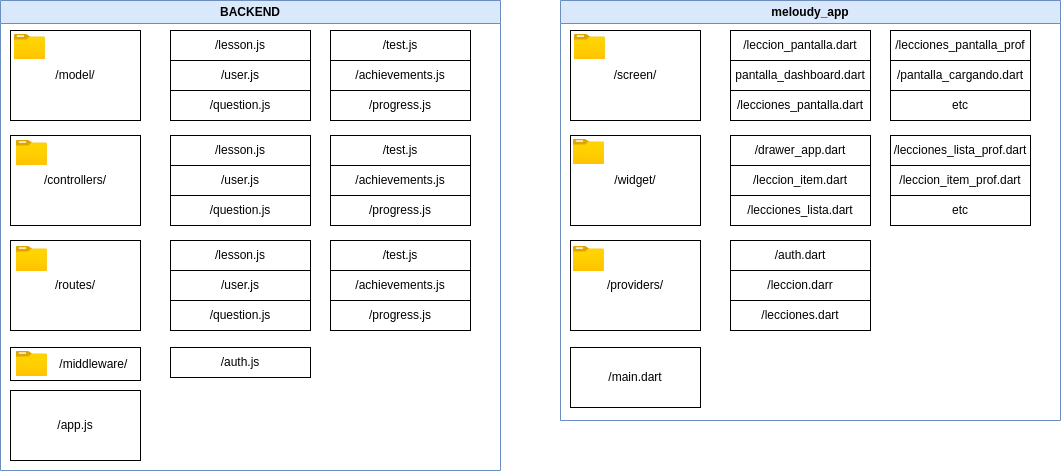
\includegraphics[width=\textwidth]{imagenes/c7/estructura.png}
  \caption{Estructura del proyecto, donde se puede ver la parte de frontend y la parte de backend.}
  \label{fig:login}
\end{figure}

En la figura anterior podemos ver que el desarrollo del proyecto se ha realizado en dos partes, una parte de frontend y otra de backend.

La parte de backend se ha desarrollado en Node.js, por lo que se han dividido los archivos en carpetas de acuerdo a su funcionalidad:
\begin{itemize}
    \item \textit{app.js}: Archivo principal de la aplicación. En él se configura el servidor y se importan las rutas.
    \item \textit{routes}: Carpeta que contiene las rutas de la API. Dentro se encuentran distintos archivos que contienen las rutas de cada entidad de la base de datos (user, lesson, question...).
    \item \textit{controllers}: Carpeta que contiene los controladores de las rutas de la API. Dentro se encuentran distintos archivos que contienen los controladores de cada entidad de la base de datos (user, lesson, question...)
    \item \textit{models}: Carpeta que contiene los modelos de la base de datos.
    \item \textit{middleware}: Carpeta que contiene los middleware de la aplicación. Por dichos middleware pasarán algunas peticiones que se hagan a la API.
\end{itemize}

La parte de frontend se ha desarrollado en Flutter, por lo que se han dividido los archivos en carpetas de acuerdo a su funcionalidad, dentro de la carpeta \textit{lib}:

\begin{itemize}
  \item \textit{main.dart}: Archivo principal de la aplicación. En él se configura la aplicación y se importan las rutas.
  \item \textit{providers}: Carpeta que contiene los providers de la aplicación. Los providers son clases que se encargan de gestionar el estado de la aplicación.
  \item \textit{screen}: Carpeta que contiene las pantallas de la aplicación. Dentro se encuentran distintos archivos que implementan cada pantalla de la aplicación.
  \item \textit{widgets}: Carpeta que contiene los widgets de la aplicación. Dentro se encuentran los archivos de los widgets que se utilizan en las distintas pantallas de la aplicación.
\end{itemize}

\section{Definición de la API (Backend)}
\label{sec:api}
En esta sección se describirá la API que se ha desarrollado para el sistema. La API se ha desarrollado en Node.js y se ha utilizado el framework Express para trabajar con el protocolo HTTP.

\subsection{Rutas}

\subsubsection{Usuarios}
\label{sec:usuarios}
La API cuenta con las siguientes rutas para la gestión de usuarios:

\begin{itemize}
    \item \textit{POST /api/user/registro}: Ruta para registrar un usuario. Recibe los datos del usuario en el cuerpo de la petición, encripta la contraseña y almacena todos los datos en la base de datos. Si el usuario se registra correctamente, se devuelve un token que se utilizará para la autenticación de las peticiones que se hagan a la API.
    \item \textit{POST /api/user/login}: Ruta para iniciar sesión. Recibe los datos del usuario en el cuerpo de la petición y comprueba si el usuario existe en la base de datos. En caso de que el usuario exista, se comprueba que la contraseña sea correcta. Si la contraseña es correcta, se devuelve un token que se utilizará para la autenticación de las peticiones que se hagan a la API.
    \item \textit{GET /api/user/get-user/\{id\}}: Ruta para obtener los datos de un usuario. Recibe por parámetro el id del usuario y devuelve los datos de dicho usuario.
    \item \textit{GET /api/user/get-users}: Ruta para obtener los datos de todos los usuarios. No recibe ningún parámetro y devuelve una lista de los datos de todos los usuarios.
%    \item \textit{PUT /api/user}: Ruta para actualizar los datos de un usuario. Recibe los datos del usuario en el cuerpo de la petición y los actualiza en la base de datos. Si el usuario se actualiza correctamente, se devuelve un token que se utilizará para la autenticación de las peticiones que se hagan a la API.
    \item \textit{DELETE /api/user/delete-user/\{id\}}: Ruta para eliminar un usuario. Recibe por parámetro el id del usuario y lo elimina de la base de datos.
    
\end{itemize}

\subsubsection{Lecciones}
\label{sec:lecciones}
La API cuenta con las siguientes rutas para la gestión de lecciones:

\begin{itemize}
    \item \textit{POST /api/lesson/create-lesson}: Ruta para crear una lección. Recibe los datos de la lección en el cuerpo de la petición y los almacena en la base de datos. Si la lección se crea correctamente, se devuelve la lección creada.
    \item \textit{GET /api/lesson/get-lessons/\{id\}}: Ruta para obtener los datos de una lección. Recibe por parámetro el id de la lección y se devuelven los datos de esta.
    \item \textit{PUT /api/lessons/:id}: Ruta para actualizar los datos de una lección. Recibe los datos de la lección en el cuerpo de la petición y los actualiza en la base de datos. Si la lección se actualiza correctamente, se devuelve la lección actualizada.
    \item \textit{DELETE /api/lessons/:id}: Ruta para eliminar una lección. Recibe el token del usuario en el encabezado de la petición y comprueba si el token es correcto. Si el token es correcto, se elimina de la base de datos la lección cuyo id coincida con el recibido.
    \item \textit{POST /api/lesson/upload-image/}: Ruta para subir una imagen de una lección al servidor. Recibe por parámetro el id de la lección y la imagen en el cuerpo de la petición.
\end{itemize}

\subsubsection{Preguntas}
\label{sec:preguntas}
La API cuenta con las siguientes rutas para la gestión de preguntas:

\begin{itemize}
  \item \textit{GET /api/question/get-questions}: Ruta para obtener todas las preguntas almacenadas en la base de datos.
  \item \textit{GET /api/question/get-questions/\{idLeccion\}}: Ruta para obtener las preguntas de una lección. Recibe por parámetro el id de la lección y devuelve todas las preguntas existentes de dicha lección.
  \item \textit{GET /api/question/get-question-test/\{idTest\}}: Ruta para obtener las preguntas de un test. Recibe por parámetro el id del test y devuelve todas las preguntas existentes de dicho test junto con el propio test.
  \item \textit{GET /api/question/get-question/\{id\}}: Ruta para obtener los datos de una pregunta. Recibe por parámetro el id de la pregunta y devuelve los datos de dicha pregunta.
\end{itemize}

\subsubsection{Tests}
\label{sec:tests}
La API cuenta con las siguientes rutas para la gestión de tests:

\begin{itemize}
  \item \textit{GET /api/progress/get-tests-progress/\{idUsuario\}/\{idLeccion\}}: Ruta para obtener todos los tests de un usuario en una lección. Recibe por parámetro el id del usuario y el de la lección, busca el progreso a partir de estos identificadores, busca todos los tests de dicho progreso y los devuelve.
\end{itemize}


\subsubsection{Progress}
\label{sec:progress}
La API cuenta con las siguientes rutas para la gestión del progreso de los usuarios:

\begin{itemize}
  \item \textit{POST /api/progress/create-test-and-progress/}: Ruta para crear un test y el progreso de un usuario. Recibe los datos del test y del progreso en el cuerpo de la petición y los almacena en la base de datos. Si el progreso ya estaba creado, solamente se almacena el nuevo test y se añade a la lista de tests del progreso. Si el test y el progreso se crean correctamente, se devuelve el test y el progreso creados. 
\end{itemize}




\subsection{Middleware}
\label{sec:middleware}
Un middleware es una función intermediaria que se utiliza para realizar acciones comunes a varias funcionalidades. La API cuenta con los siguientes middleware:

\begin{itemize}
  \item \textit{auth}: Middleware que comprueba si el token del usuario es correcto (es decir, si el usuario está identificado en la aplicación).
   Si el token es correcto, se pasa a la siguiente función. Si el token no es correcto, se devuelve un error.
\end {itemize}

A continuación se explicarán todas las pantallas y funcionalidades de la aplicación. Para cada una de ellas se explicará la vista y la lógica de la misma. 
Para la vista, se mostrará una captura de pantalla de la pantalla en cuestión y un diagrama de la estructura de widgets que se han utilizado para construir la pantalla. 
Este diagrama detallará los principales widgets utilizados en cada vista. \textit{Cabe destacar que en algunas pantallas se han omitido algunos widgets para simplificar 
el diagrama y se han utilizado los nombres "C1, C2, C3..." para referirse a los hijos del widget distribuidor en columna (Column) y "F1, F2, F3..." para referirse a los hijos
 del widget distribuidor en fila (Row).}
\newpage


\section{Funcionalidad de inicio}
\label{sec:inicio}
A continuación presentamos la funcionalidad básica de la aplicación que usará cualquier usuario que se registre:


% \subsection{Pantallas y Widgets básicos}
% \label{sec:widgets}
% La aplicación cuenta con una serie de pantallas y widgets que se utilizan en todas las pantallas de la aplicación. 
% Estos widgets se han desarrollado para que se puedan reutilizar en las distintas pantallas de la aplicación. A continuación se describen los widgets y pantallas que se han desarrollado:


\subsection{Drawer}
Un drawer es un menú lateral que se puede abrir y cerrar y que se utiliza para acceder a distintas pantallas de la aplicación. En este caso, se
abre y se cierra clickando en el icono superior izquierdo de la aplicación. Se ha utilizado el llamado "menú hamburguesa". En la siguiente imagen se puede ver el drawer abierto:

\begin{figure}[H]
    \centering
    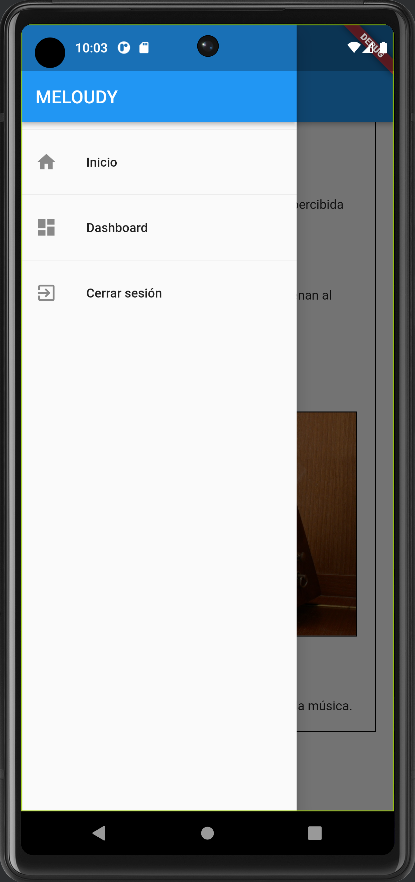
\includegraphics[width=0.4\textwidth]{imagenes/c7/drawer.png}
    \caption{Drawer abierto en la aplicación con tres opciones (por ser desde la vista del profesor): Inicio, Dashboard y Cerrar sesión.}
    \label{fig:drawer}
\end{figure}


\subsection{Sesión}
\label{sec:sesion}
Se han desarrollado tres características adicionales relacionadas con la sesión de usuario y que explicaremos con más detalle en cada uno de los apartados de la sesión.
\begin{itemize}
    \item \textbf{Encriptación de la contraseña:} La contraseña del usuario se encripta antes de ser almacenada en la base de datos para evitar que sea
     visible por cualquier persona que tenga acceso a esta. De esta forma garantizamos que se cumple el requisito de seguridad de la contraseña. 
     Para esto se ha utilizado un algoritmo hash de la biblioteca \textit{bcrypt}.
    El diagrama que explica el proceso de encriptación se muestra en la siguiente imagen:
    \begin{figure}[H]
      \centering
      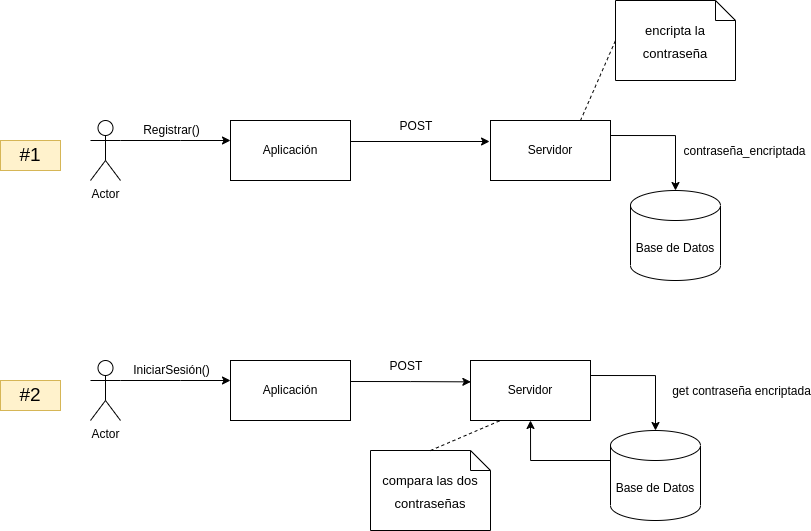
\includegraphics[width=0.9\textwidth]{imagenes/c7/logindiag.png}
      \caption{Diagrama que explica el proceso de encriptación en el inicio de sesión desarrollado en la aplicación.}
      \label{fig:login}
    \end{figure}

    \item \textbf{Intercambio de token:} El servidor proporciona un token al usuario cuando se registra o inicia sesión. Este token se añade a las peticiones 
    que se hagan a la API. De esta forma, garantizamos que se cumple el requisito de seguridad de la sesión y 
    que todas las peticiones válidas que se hagan a la API son de usuarios registrados. Además, el token fija una fecha de expiración al crearse para aumentar
     la seguridad del usuario. Esta funcionalidad se ha logrado con el paquete \textit{jsonwebtoken} de NodeJS ~\cite{JWT}.
    El diagrama que explica el proceso de intercambio de token se muestra en la siguiente imagen:

    \begin{figure}[H]
      \centering
      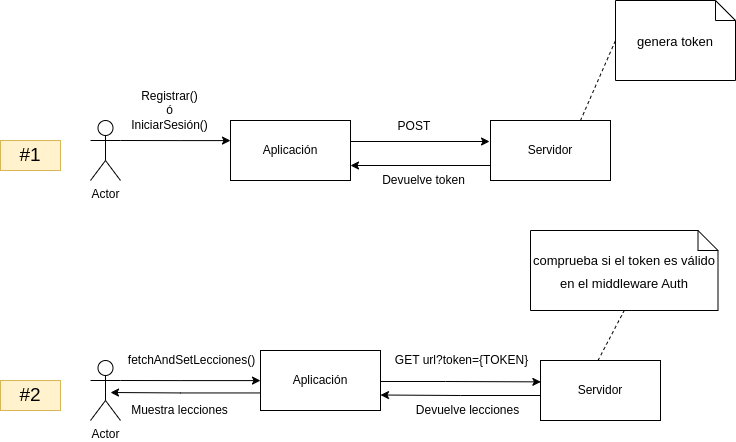
\includegraphics[width=0.9\textwidth]{imagenes/c7/tokendiag.png}
      \caption{Diagrama que explica el proceso de intercambio de token en el inicio de sesión desarrollado en la aplicación.}
      \label{fig:token}
    \end{figure}

    \item \textbf{Sesión entre instancias:} La sesión se mantiene entre instancias de la aplicación. Es decir, si el usuario cierra la aplicación y 
    la vuelve a abrir, no tendrá que volver a iniciar sesión si no ha cerrado la sesión o si el token no ha expirado. 
    Esto se ha conseguido mediante el almacenamiento del token en la memoria local del dispositivo con la biblioteca \textit{shared\_preferences} ~\cite{sharedpreferences}.
    De esta forma, cuando el usuario inicia sesión, el token se almacena en el almacenamiento local del dispositivo 
    y cuando el usuario cierra la aplicación y la vuelve a abrir, el token se recupera del almacenamiento local del dispositivo y se comprueba si es correcto. 
    Si es correcto, se pasa a la siguiente pantalla. Si no es correcto, se vuelve a la pantalla de inicio de sesión.
    Este token además estará siendo comprobado constantemente para que si el este expira, se cierre la sesión y se vuelva a la pantalla de inicio de sesión evitando accesos no autorizados.

    El diagrama que explica el proceso de sesión entre instancias se muestra en la siguiente imagen:

    \begin{figure}[H]
      \centering
      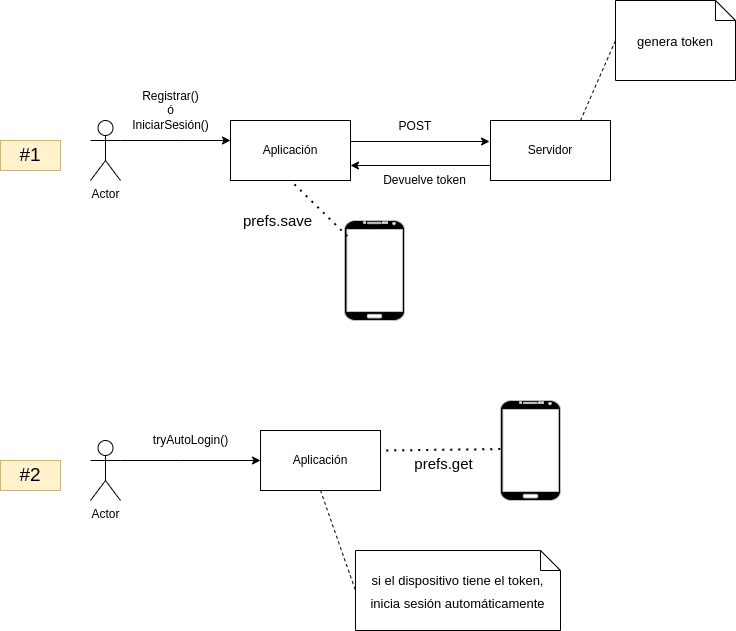
\includegraphics[width=0.9\textwidth]{imagenes/c7/token2.png}
      \caption{Diagrama que explica el proceso de sesión entre instancias en el inicio de sesión desarrollado en la aplicación.}
      \label{fig:sesion}

    \end{figure}

  \end{itemize}

\subsubsection{Inicio de sesión}
\textit{Desarrollado en el Sprint 5}
\label{sec:login}

La aplicación cuenta con una pantalla de inicio de sesión para que los usuarios puedan acceder a la aplicación con su cuenta registrada previamente. 
Para el inicio de sesión, el usuario deberá introducir su nombre de usuario y su contraseña. 
Si el usuario no tiene una cuenta, podrá registrarse pulsando en el botón 'Registrarse'. En la siguiente imagen se puede ver la pantalla de inicio de sesión:

\begin{figure}[H]%
  \centering
  \subfloat[\centering Pantalla de login]{{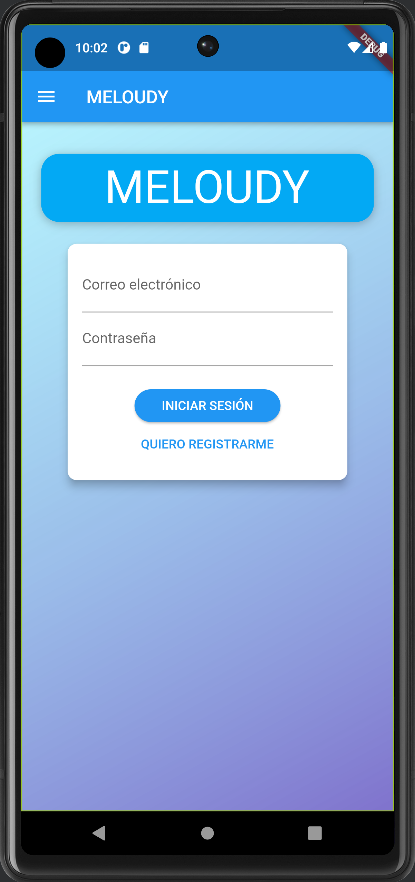
\includegraphics[width=0.40\textwidth]{imagenes/c7/login.png} }}%
  \qquad
  \subfloat[\centering Estructura en componentes de la pantalla de login.]{{ 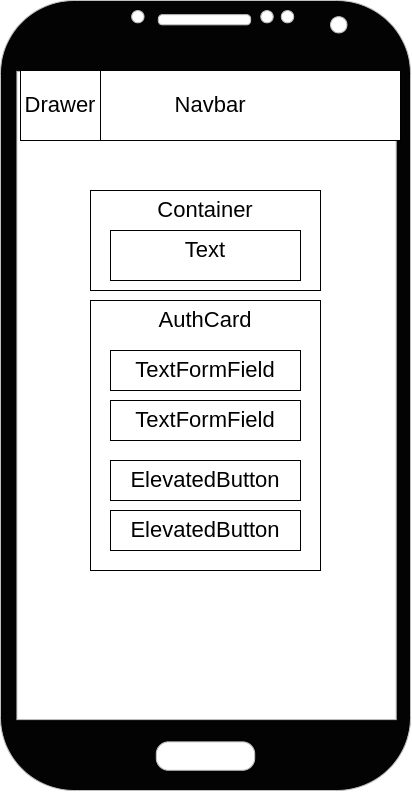
\includegraphics[width=0.406\textwidth]{imagenes/c7/logincompo.png} }}%
  \caption{Pantalla de inicio de sesión del usuario donde se puede ver el formulario de inicio de sesión con los campos de usuario (correo) y contraseña.}%
  \label{fig:login}%
\end{figure}


\paragraph*{Vista}
Empezando por la vista, se ha desarrollado un widget para la pantalla de inicio de sesión. Este widget se compone de un formulario con dos 
campos de texto, uno para el nombre de usuario y otro para la contraseña. Además, el formulario contiene un botón para iniciar sesión y otro 
para ir a registrarse si el usuario así lo desea.

La pantalla tiene una pila que contiene dos widgets: un container con un fondo en degradado conseguido con el atributo \textit{gradient} de la 
clase \textit{BoxDecoration} de Flutter, y un SingleChildScrollView que consta de un widget Column para poder colocar los elementos de forma vertical. 
Dichos elementos son: un \textit{Container} para el título de la aplicación y un Widget personalizado que contiene el formulario de inicio de sesión \textit{AuthCard()}.

Este último no es más que un widget de la clase \textit{Card} con dos \textit{TextFormField} (uno para el correo electrónico y otro para la contraseña) 
y un \textit{ElevatedButton} para proceder al inicio de sesión.

\paragraph*{Lógica}
En cuanto a la lógica, una vez el cliente pulsa el botón de 'Iniciar sesión', se llama a la función asíncrona \textit{submit}, 
la cual se encarga de comprobar que los datos introducidos son correctos.
Cuando los datos son comprobados, se procede a iniciar sesión en la aplicación mediante el método de inicio de sesión del Provider Auth.
 Para esto, se envia una petición HTTP POST a la ruta \textit{/user/login} de la API con los datos escritos en el formulario de inicio de sesión.

Por otro lado, en el servidor cuando la petición es recibida a dicha ruta, se ejecuta una función en el controlador para el inicio de sesión de usuarios.
 Esta función capta los valores y comprueba que el usuario existe en la base de datos. Si el usuario existe, se comprueba que la contraseña introducida es correcta mediante el método \textit{verify} de bcrypt. Si los datos son correctos, se genera el token de sesión y se devuelve al cliente. Si el usuario no existe o la contraseña es incorrecta, se devuelve un código de estado 400 y un mensaje de error.

Cuando el cliente recibe la respuesta del servidor, se comprueba si el código de estado es 200, lo que significa que el inicio de sesión ha sido correcto.
 En este caso, se almacena el token de sesión en el dispositivo tal y como se ha explica en la sección \ref{sec:sesion}. 

 \newpage
\subsubsection{Registro}
\textit{Desarrollado en el Sprint 5}
\label{sec:register}

La aplicación cuenta con una pantalla de registro para que los usuarios puedan registrarse en la aplicación. 
Para el registro, el usuario deberá introducir su nombre de usuario y su contraseña dos veces. Si el usuario ya tiene una cuenta,
 podrá iniciar sesión pulsando en el botón 'Iniciar sesión'. En la siguiente imagen se puede ver la pantalla de registro:



\paragraph*{Vista}
La vista del registro es muy similar a la del inicio de sesión. La única diferencia es que el formulario contiene 
un campo adicional para introducir la contraseña otra vez por razones de seguridad.

\begin{figure}[H]
  \centering
  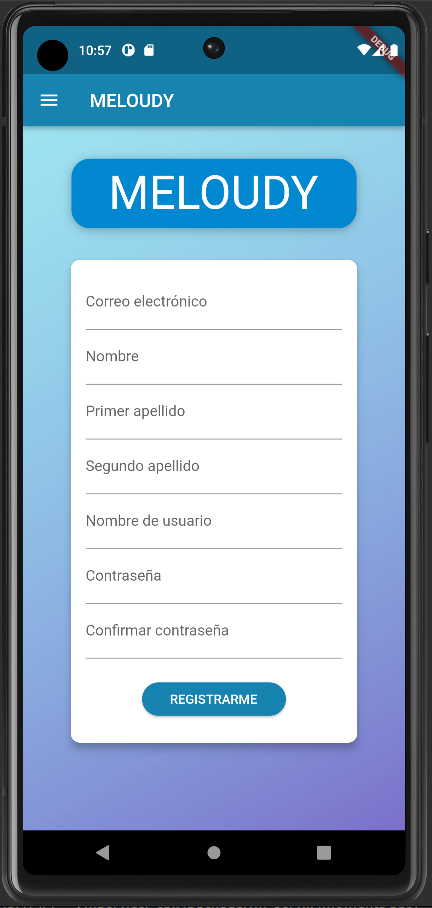
\includegraphics[width=0.4\textwidth]{imagenes/c7/registro.png}
  \caption{Pantalla de registro de los usuarios donde se puede ver el formulario de registro con los campos de usuario (correo), contraseña y repetir la contraseña.}
  \label{fig:register}
\end{figure}


\paragraph*{Lógica}
En cuanto a la lógica, una vez el cliente pulsa el botón de 'Registrarse', también se llama a la función asíncrona \textit{submit}, que se encarga de comprobar que los datos introducidos 
son correctos. Cuando se ha hecho esto, si los datos son válidos, la función llama al método de registro del Provider Auth, 
el cual envia una petición HTTP POST a la ruta \textit{/user/registro} de la API con los datos escritos en el formulario de registro. 

Para poder procesar esta petición de Flutter, una vez el servidor recibe la petición a la ruta de registro, se ejecuta una función en el controlador para el registro de usuarios.
 Esta función capta los valores, encripta la contraseña y crea el usuario en la base de datos. Si los datos son correctos, se genera un token de sesión y
  se devuelve al cliente junto con un código de estado 201 y un mensaje de éxito. Si el registro no es correcto, se devuelve un código de estado 400 y un mensaje de error.

  Cuando Flutter recibe la respuesta del servidor, almacena el token de sesión en el dispositivo tal y como se ha explica en la sección \ref{sec:sesion}.

\subsubsection{Cierre de sesión}
\textit{Desarrollado en el Sprint 5}
\label{sec:logout}

La aplicación cuenta con una opción para cerrar sesión. Para cerrar sesión, el usuario deberá pulsar en el botón \textit{Cerrar sesión}
 que se encuentra en el drawer (barra lateral) de la aplicación. También se cerrará sesión automáticamente si el token ha expirado.

\paragraph*{Vista}
Para el cierre de sesión, se ha añadido una fila al drawer (barra lateral) de la aplicación, el cual el usuario clicará cuando desee cerrar su sesión.

\paragraph*{Lógica}
La lógica del cierre de sesión es sencilla: se llama a la función \textit{logout} de la clase \textit{Auth} donde se restablecen 
los valores de la sesión y se limpian los datos de la sesión almacenados en el dispositivo con el paquete \textit{shared\_preferences}. 
Esta limpieza de datos se realiza en el método \textit{clear}.
Además, se ha añadido un timer que se encarga de cerrar la sesión automáticamente si el token ha expirado. Este timer se ejecuta 
cada cierto tiempo y comprueba si el token ha expirado. Si es así, se llama al método \textit{logout} mencionado anteriormente.

\newpage

\section{Funcionalidad de usuario}
\label{sec:funcionalidad_usuario}


\subsection{Lista de lecciones}
\textit{Desarrollado en el Sprint 5}
\label{sec:lista_lecciones}

La aplicación cuenta con una lista de lecciones que el usuario puede ver. Esta lista es la pantalla inicial de la aplicación y el usuario 
la visualizará al iniciar sesión. También puede acceder a ella pulsando el botón \textit{Inicio} que se encuentra en el drawer (barra lateral) de la aplicación.


\begin{figure}[H]%
  \centering
  \subfloat[\centering Pantalla de lecciones]{{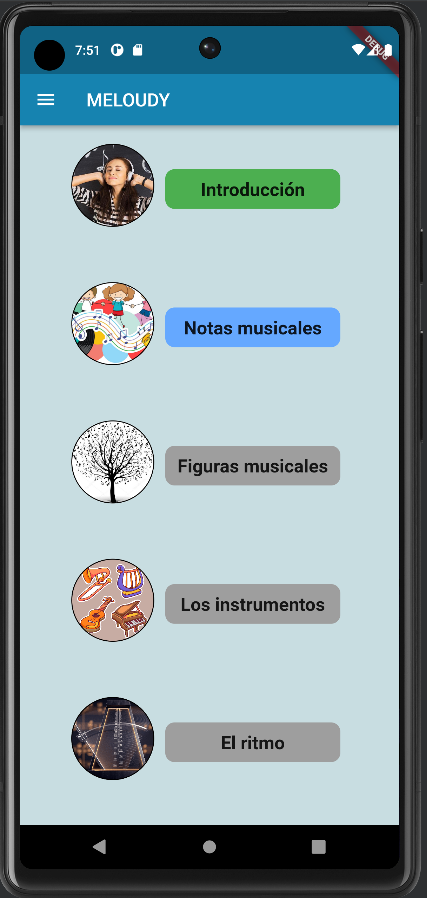
\includegraphics[width=0.45\textwidth]{imagenes/c7/pantprin.png} }}%
  \qquad
  \subfloat[\centering Estructura en componentes de la pantalla de lecciones.]{{ 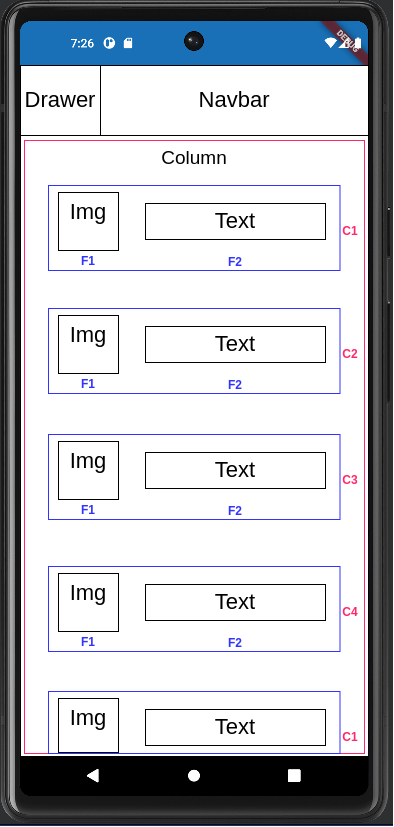
\includegraphics[width=0.45\textwidth]{imagenes/c7/listaleccionescompo.png} }}%
  \caption{Pantalla de la lista de lecciones con el título y la imagen de cada lección.}%
  \label{fig:login}%
\end{figure}

\newpage

\paragraph*{Vista}
Para que el usuario pueda ver la lista de lecciones, se ha desarrollado un widget principal para la pantalla. Este widget contiene el widget \textit{ListaLecciones}, 
que contiene un componente para la distribución de widgets en una columna. Cada uno de estos widgets se llama \textit{LeccionItem} y contendrá la
 información principal de una lección, como el título y la imagen de perfil. En la figura anterior se puede ver la pantalla de lista de lecciones.

\paragraph*{Lógica}
Para la lógica de esta pantalla se ha utilizado el patrón de diseño \textit{Provider} para la gestión de estados. Un provider es un objeto que se 
encarga de gestionar el estado de la aplicación y proporcionarselo a los widgets que lo necesiten.
En este caso, se ha utilizado para gestionar el estado de la lista de lecciones y se le ha llamado \textit{Lecciones}.
Este Provider se encarga de obtener la lista de lecciones de la API (llamada HTTP con el verbo GET a la ruta (\textit{GET /api/lesson/get-lessons/\{id\}}))
 y almacenar cada uno de sus elementos en variables de la clase \textit{Lección}. Además, se ha creado un método público que devuelve la lista de lecciones. 
 Este método se utiliza en el widget \textit{ListaLecciones} para obtener la lista de lecciones, añadir cada lección en forma de widget de forma iterativa
 y mostrarla en pantalla. 

\subsection{Ver lección} 
\textit{Desarrollado en el Sprint 5}
\label{sec:leccion}

La aplicación cuenta con una vista para cada lección. Esta vista se puede acceder pulsando en el título o en la imagen de una lección en la lista de lecciones.
 En esta vista se puede ver el contenido de la lección, como el título, el texto, las imágenes, los vídeos, etc.
Además, al final de la lección se puede hacer un test para comprobar los conocimientos adquiridos y revisar los tests realizados anteriormente por el usuario.

\begin{figure}[H]%
  \centering
  \subfloat[\centering Parte 1.]{{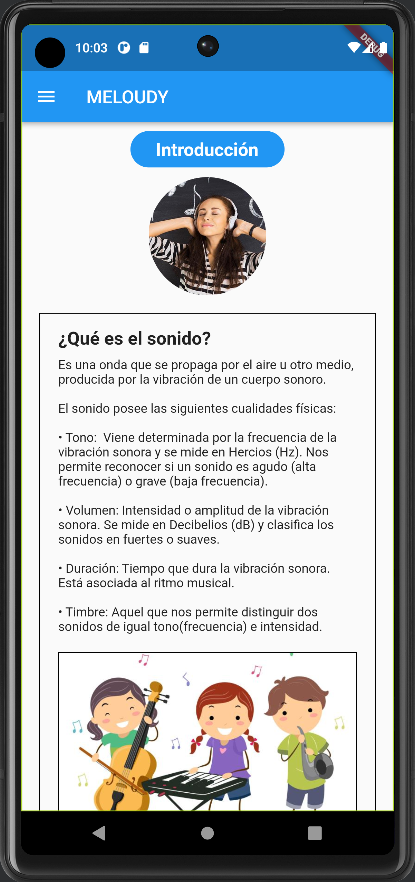
\includegraphics[width=0.38\textwidth]{imagenes/c7/leccion.png} }}%
  \qquad
  \subfloat[\centering Parte 2.]{{ 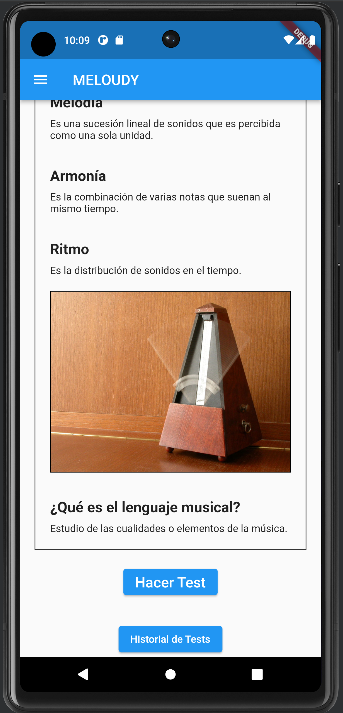
\includegraphics[width=0.38\textwidth]{imagenes/c7/leccion2.png} }}%
  \caption{Pantalla de una lección en concreto con los contenidos (títulos, texto, multimedia...) del temario y los dos botones relacionados con los tests.}%
  \label{fig:example}%
\end{figure}

\paragraph*{Vista}
La vista de una lección proporciona al usuario información más detallada de esta. En primer lugar se muestra la imagen de la lección y el título 
en un componente para distribuir widgets en una fila. (Un widget \textit{Row} compuesto de un \textit{Text} y un \textit{Image} ).
A continuación, se muestra el contenido de la lección en forma de texto, imágenes, vídeos, etc. Esto se ha conseguido construyendo 
widgets de forma dinámica dependiendo del tipo de contenido almacenado y añadiéndolos a un widget distribuidor en columna (\textit{Column}).
Finalmente, se muestra un botón en pantalla para poder hacer un test y otro para ver el historial de tests realizados, ambos mediante un widget \textit{ElevatedButton}.
En la siguiente imagen se puede ver la pantalla de una lección:

\begin{figure}[H]%
  \centering
  \subfloat[\centering Parte 1.]{{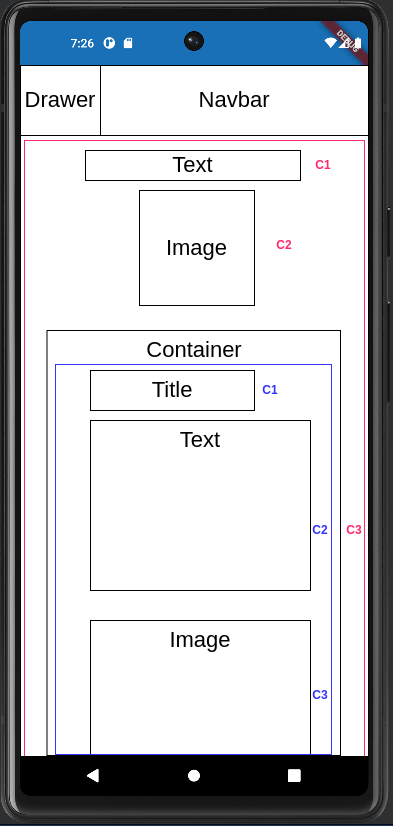
\includegraphics[width=0.38\textwidth]{imagenes/c7/leccioncompo.png} }}%
  \qquad
  \subfloat[\centering Parte 2.]{{ 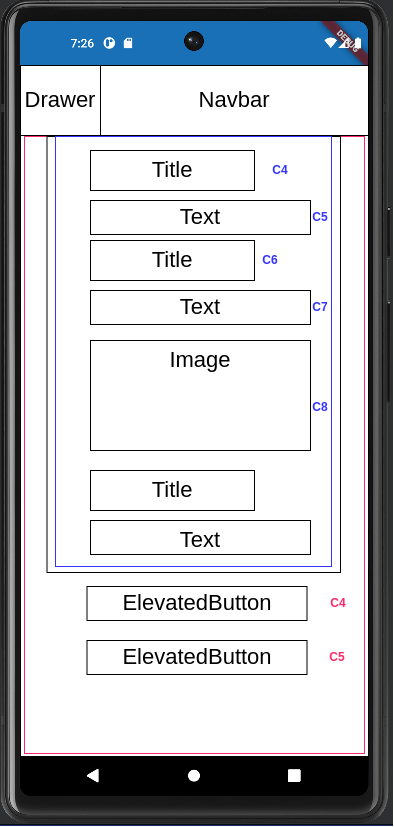
\includegraphics[width=0.38\textwidth]{imagenes/c7/leccioncompo2.png} }}%
  \caption{Pantalla de una lección en concreto con los contenidos (títulos, texto, multimedia...) del temario y los dos botones relacionados con los tests.}%
  \label{fig:example}%
\end{figure}




\paragraph*{Lógica}
Para la lógica de esta pantalla se ha utilizado el provider \textit{Lecciones} mencionado anteriormente. En este caso, el provider se encarga 
de obtener la lección que se quiere mostrar en pantalla de la lista de lecciones y devolverla al widget que la mostrará en pantalla.
Además, se ha implementado una funcionalidad para poder construir el constenido de la lección de forma dinámica.
 Para esto se ha realizado un bucle que recorre el contenido de la lección y dependiendo del tipo de contenido, se construye un widget diferente. 
 Por ejemplo, si el contenido es un texto, se construye un widget \textit{Text} y se añade a la lista de widgets que se devolverán al final del método. 
 Si el contenido es una imagen, se construye un widget \textit{Image} y se añade a la lista de widgets que se devolverán al final del método. De esta forma 
se consigue que el contenido de la lección se muestre en pantalla en función del tipo y facilitaremos la adición de contenido a cada lección por parte del profesor en un futuro.

\subsection{Test}
\label{sec:test}
\textit{Desarrollado en el Sprint 6}

La lección contiene un test que se puede realizar al final de la lección. Este test consta de una serie de preguntas que el usuario deberá responder.

El usuario podrá responder a las preguntas de la siguiente forma: seleccionando una opción de la lista de opciones, seleccionando varias, 
escribiendo una respuesta en un campo de texto... El usuario podrá responder la opción que desee y pasar a la siguiente pregunta.
 A continuación se muestran las diferentes preguntas que se pueden realizar en el test.


\paragraph*{Vista}
La vista de un test consiste en una serie de preguntas que el usuario deberá responder. Al seleccionar el botón de \textit{Hacer Test} 
ubicado en la pantalla de la lección, se muestra la pantalla de un test. En esta pantalla se presenta una pregunta a la vez, y el usuario deberá responderla. 
Para pasar a la siguiente pregunta, pulsará la flecha ubicada a la derecha de la imagen y para retroceder a la pregunta anterior, pulsará la flecha izquierda.
Esto se ha realizado mediante un widget que distribuye otros widget de forma horizontal en una fila (\textit{Row}). 
Este widget se encarga de mostrar la imagen de la pregunta actual y las flechas para pasar a la siguiente o anterior pregunta.

Debajo de lo anterior, se mostrará la pregunta actual y las opciones de respuesta. Esto se ha realizado mediante un widget que distribuye
 otros widget de forma vertical en una columna (\textit{Column}). Las opciones de respuesta dependerán del tipo de pregunta que se esté mostrando. 
 Por ejemplo, si la pregunta es de selección única o múltiple, se muestra una lista de opciones de respuesta, mientras que si la pregunta es de entrada de texto,
  se muestra un campo de texto para que el usuario escriba su respuesta.

En la última pregunta, aparece un botón para enviar las respuestas y ver el resultado del test. 
Dicho botón evita que el usuario no pueda enviar las respuestas antes de responder o pasar por todas las preguntas.

\paragraph*{Lógica}
Para la lógica de esta pantalla se ha utilizado el patrón de diseño \textit{Provider} para la gestión del estado del test en curso.
Este Provider se encarga de obtener todas las preguntas del test de la API y almacenarlas en una lista privada.
 Para recorrer las preguntas, se ha utilizado un índice que se incrementa o decrementa en función de si el usuario quiere pasar a la siguiente o a la anterior pregunta. 
 Este índice se almacena también en una variable privada e irá aumentando o disminuyendo en función de si el usuario quiere pasar a la siguiente pregunta o volver a la anterior.
Cada vez que el usuario responde una pregunta, se almacenan las respuestas en una variable privada para conservarlas durante toda la navegación del test 
(si vuelve para atrás, por ejemplo) y se produce una retroalimentación al usuario cambiando el color de la opción a un azul más oscuro para que el usuario sepa qué opción ha respondido.

Cuando el usuario pulsa el botón de enviar respuestas, estas se envían al servidor para crear el test y añadirlo al progreso (se envía la petición HTTP
 a la ruta de la API \textit{POST /api/progress/create-test-and-progress/}:) y aparece la pantalla para ver el resultado del test.


\newpage 

\subsubsection{Pregunta de selección única.}\mbox{}\\

\label{sec:pregunic1}
\textit{Desarrollado en el Sprint 6}

A continuación se muestra la pantalla de una pregunta de selección única, en la que el usuario deberá seleccionar una opción de la lista de opciones:

\begin{figure}[H]%
  \centering
  \subfloat[\centering Selección única sin una respuesta seleccionada.]{{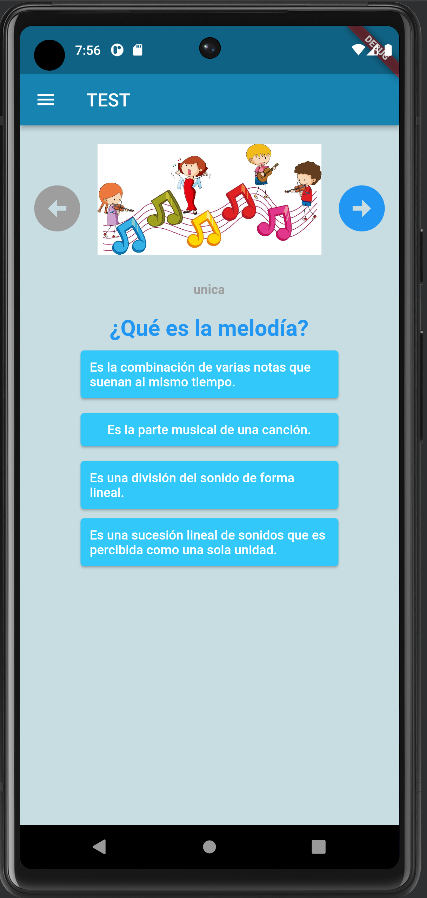
\includegraphics[width=0.45\textwidth]{imagenes/c7/selecunica.png} }}%
  \qquad
  \subfloat[\centering Selección única con una respuesta seleccionada.]{{ 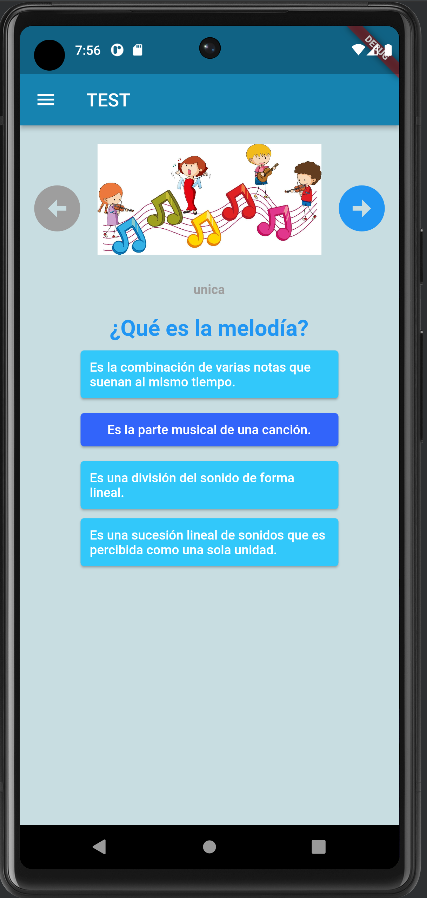
\includegraphics[width=0.45\textwidth]{imagenes/c7/selecunica2.png} }}%
  \caption{Pantalla de una pregunta de selección única en la que las opciones se muestran en forma de lista.}%
  \label{fig:example}%
\end{figure}

\newpage

\subsubsection{Pregunta de selección múltiple}\mbox{}\\

\label{sec:pregunic1}
\textit{Desarrollado en el Sprint 6}

A continuación se muestra la pantalla de una pregunta de selección múltiple, en la que el usuario deberá seleccionar una o varias opciones de la lista de opciones:

\begin{figure}[H]%
  \centering
  \subfloat[\centering Selección múltiple sin una respuesta seleccionada.]{{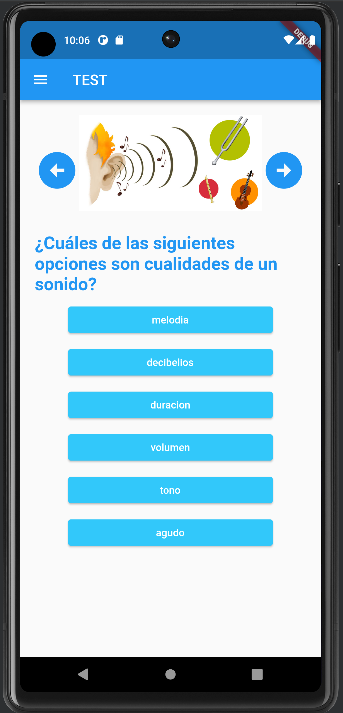
\includegraphics[width=0.45\textwidth]{imagenes/c7/selecmulti.png} }}%
  \qquad
  \subfloat[\centering Selección múltiple con varias respuestas seleccionadas.]{{ 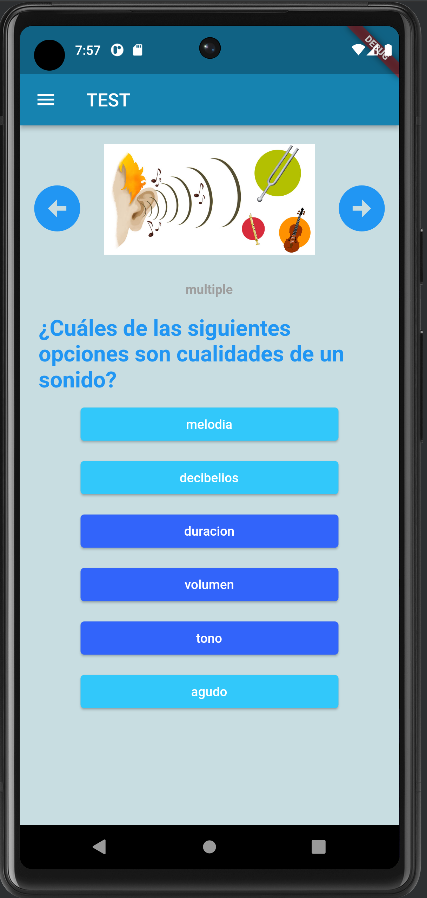
\includegraphics[width=0.45\textwidth]{imagenes/c7/selecmulti2.png} }}%
  \caption{Pantalla de una pregunta de selección múltiple en la que las opciones se muestran en forma de lista.}%
  \label{fig:example}%
\end{figure}



\newpage

\subsubsection{Pregunta de entrada de texto}

\label{sec:pregunic1}
\textit{Desarrollado en el Sprint 6}

A continuación se muestra la pantalla de una pregunta de entrada de texto, en la que el usuario deberá escribir la respuesta en un campo de texto:

\begin{figure}[H]%
  \centering
  \subfloat[\centering Entrada de texto sin respuesta introducida.]{{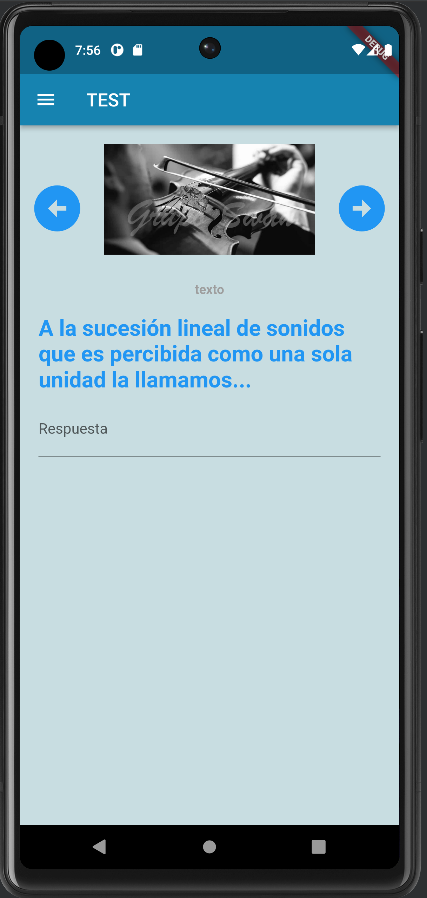
\includegraphics[width=0.45\textwidth]{imagenes/c7/entradatexto.png} }}%
  \qquad
  \subfloat[\centering Entrada de texto con respuesta introducida.]{{ 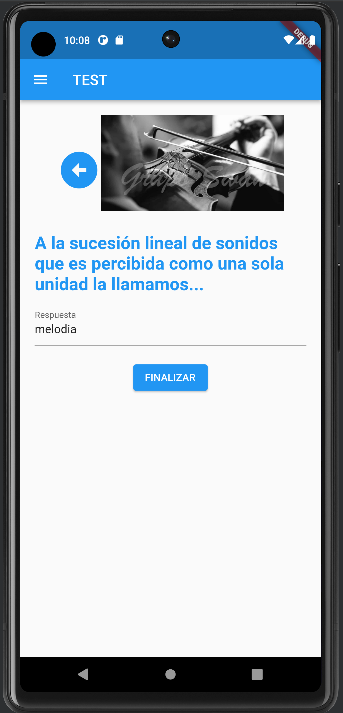
\includegraphics[width=0.45\textwidth]{imagenes/c7/entradatexto2.png} }}%
  \caption{Pantalla de una pregunta de entrada de texto. }%
  \label{fig:example}%
\end{figure}

\newpage
\subsubsection{Pregunta de micrófono}

\label{sec:pregunic1}
\textit{Desarrollado en el Sprint 7}

A continuación se muestra la pantalla de una pregunta de micrófono, en la que el usuario deberá grabar la respuesta mediante el micrófono del dispositivo. Esta respuesta
debe ser fiel a la partitura que se muestra en la imagen de la pregunta. 

\begin{figure}[H]%
  \centering
  \subfloat[\centering Pregunta de micrófono sin respuesta introducida.]{{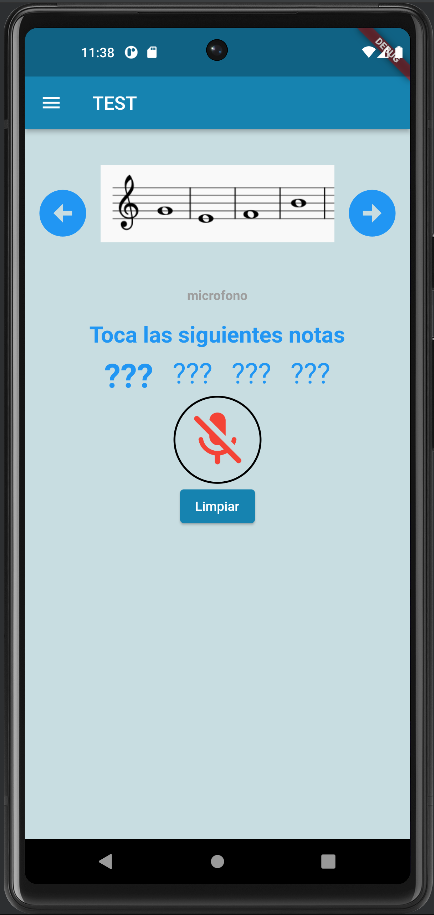
\includegraphics[width=0.45\textwidth]{imagenes/c7/entradamicrofono.png} }}%
  \qquad
  \subfloat[\centering Pregunta de micrófono introduciendo respuesta.]{{ 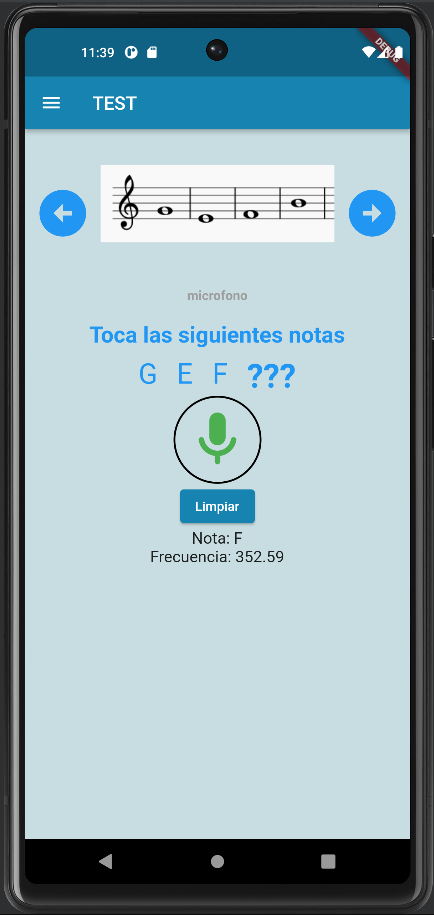
\includegraphics[width=0.45\textwidth]{imagenes/c7/entradamicrofono2.png} }}%
  \caption{Pantallas de una pregunta de micrófono. }%
  \label{fig:example}%
\end{figure}

\begin{figure}[H]
  \centering
  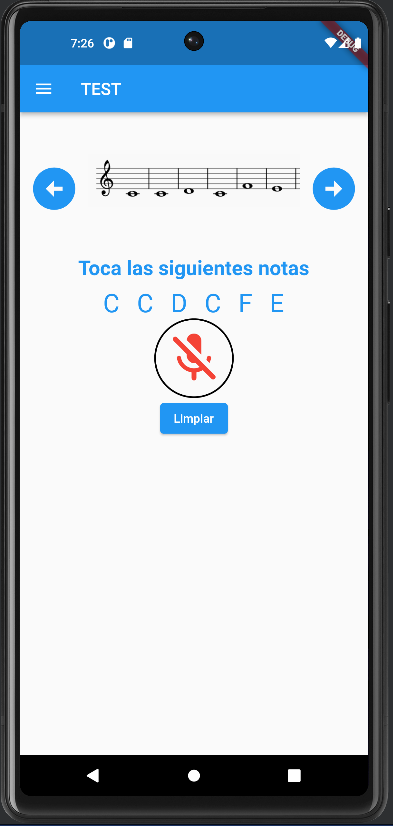
\includegraphics[width=0.37\textwidth]{imagenes/c7/entradamicrofono3.png}
  \caption{Pregunta de micrófono con respuesta introducida.}
  \label{fig:login}
\end{figure}

\paragraph*{Lógica}
Para realizar la lógica de esta pantalla se ha utilizado la biblioteca \textit{flutter\_fft}, que utiliza la transformada de Fourier de una señal de audio para obtener la frecuencia que se utiliza para determinar el tono del sonido,
 y obtener la nota musical que se está reproduciendo a partir de dicho valor de frecuencia ~\cite{fft}.
Para ello, la biblioteca utiliza un \textit{StreamBuilder} que se encarga de obtener la frecuencia de la señal de audio. 
Se han realizado algunas modificaciones al código de la biblioteca para que la detección de notas sea más precisa y
 se pueda obtener la nota musical real que se está reproduciendo (había cierto desajuste que detectaba medio semitono más de lo que se estaba tocando).

Cabe mencionar que \textit{flutter\_fft} se le pueden ajustar varios parámetros para que la detección de notas sea más o menos precisa, 
como el número de muestras que se toman por segundo, el intervalo entre muestras, etc.

Cuando el usuario pulsa el botón del micrófono, se inicia el \textit{StreamBuilder}, se cambia el estado del widget para establecer 
que se está grabando (variable isRecording) y se muestra una retroalimentación al usuario cambiando el color del botón para notificar al usuario.

Además, las notas musicales se muestran en pantalla conforme el algoritmo las identifica. De esta manera, el usuario puede comprobar la exactitud de su interpretación en tiempo real.
Cuando se completan todas las notas de la partitura, se detiene el \textit{StreamBuilder} automáticamente.
Además, en el momento en el que el usuario pulsa el botón del micrófono cuando esté esta grabando, también se detiene el \textit{StreamBuilder}.

Si el usuario no está conforme con la respuesta, puede pulsar el botón de ``Reiniciar'' para resetear el ejercicio y puede volver a grabar pulsando el botón de micrófono. 
Por otro lado, si está conforme, puede pulsar el botón de siguiente para pasar a la siguiente pregunta.

\subsubsection{Resultado del test}
\label{sec:pregunta}
\textit{Desarrollado en el Sprint 6}

A continuación se muestra la pantalla de resultado del test, en la que se muestra el número y el porcentaje de aciertos respecto a las preguntas. 
Además, se muestra una barra de progreso que muestra el porcentaje de aciertos respecto al número de preguntas preguntas. (Figura \ref{fig:fin_test})

\begin{figure}[H]%
  \centering
  \subfloat[\centering Resultado aprobado (50\% o más).]{{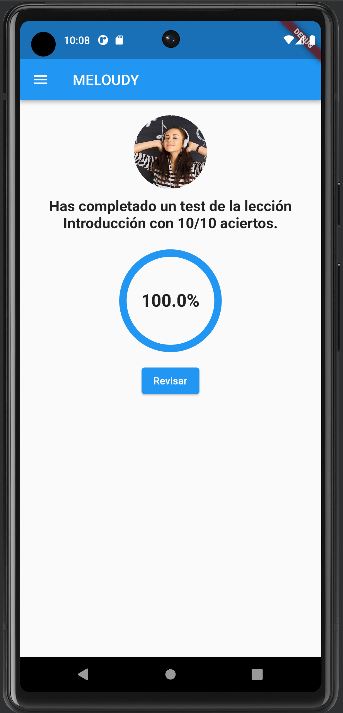
\includegraphics[width=0.37\textwidth]{imagenes/c7/porcentaje.png} }}%
  \qquad
  \subfloat[\centering Resultado suspenso (menos del 50\%).]{{ 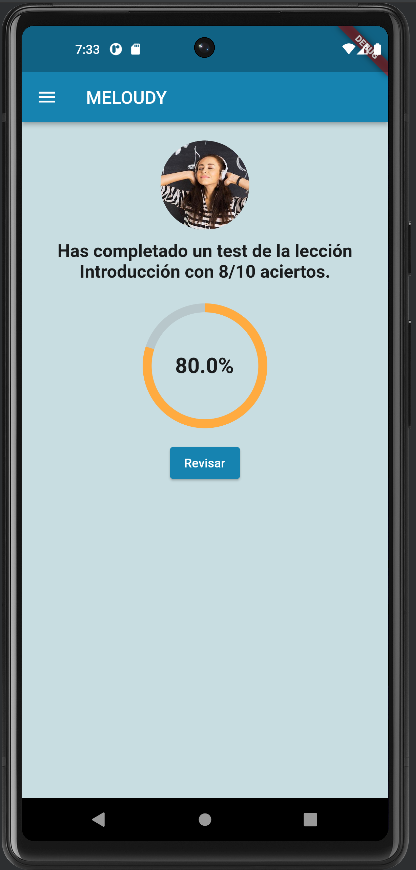
\includegraphics[width=0.37\textwidth]{imagenes/c7/porcentaje2.png} }}%
  \caption{Pantalla que muestra el resultado del test con el número de aciertos y el porcentaje de aciertos respecto a las preguntas con un Progress Bar.}%
  \label{fig:fin_test}%
\end{figure}

\paragraph*{Vista}
\label{sec:vista}

Para realizar la vista de la pantalla se ha utilizado de nuevo el widget \textit{Column} para poder mostrar los elementos de la pantalla de forma vertical. 
Dentro de dicho widget tendremos:
\begin{itemize}
  \item la imagen de la lección (widget \textit{Image}).
  \item un campo de texto para mostrar el número de aciertos (widget \textit{Text}).
  \item una barra de progreso para mostrar el porcentaje de aciertos (widget \textit{CircularPercentIndicator}). 
  Para este test se ha utilizado la biblioteca de flutter \textit{percent\_indicator}.
  \item un botón para poder revisar el test (widget \textit{ElevatedButton}).
\end{itemize}

\paragraph*{Lógica}
\label{sec:logica}
La lógica para mostrar el resultado del test es bastante sencilla.
Tras el envío del test al servidor, se comparan las respuestas del usuario con las respuestas correctas almacenadas en cada una de las preguntas 
(estas últimas se obtienen mediante el Provider de las preguntas). 
Una vez obtenidos estos datos, se calcula el porcentaje de aciertos y se envía a la vista.



\subsection{Revisar pregunta}
\label{sec:pregunta}
El usuario podrá revisar las preguntas que haya contestado en un test. Como se puede ver en la pantalla anterior del resultado del test, 
existe un botón para poder revisarlo. El usuario podrá ver las preguntas que haya contestado y las respuestas que haya seleccionado con la validación de estas.

\paragraph*{Vista}
\label{sec:vista}
La vista de la pantalla de revisión de preguntas es muy similar a la vista de la pantalla de la pregunta. 
La diferencia es que se muestran las respuestas que ha seleccionado el usuario si son correctas o no.
Por tanto, solo se han cambiado los colores de los botones y de los textos para mostrar si la respuesta es correcta o no.

\paragraph*{Lógica}
\label{sec:logica}
La lógica para mostrar la revisión de las preguntas se ha realizado comparando las respuestas del usuario con las respuestas correctas almacenadas
 en cada una de las preguntas (estas últimas se obtienen mediante el Provider de las preguntas).

Para mostrar si la respuesta es correcta o no, se ha cambiado el color del botón o del campo de texto. Si la respuesta es correcta, 
se muestra en verde y, si es incorrecta, se muestra en rojo. 

Para la validación, se ha llamado a la función \textit{validarRespuesta} que se ha creado en la clase provider \textit{Preguntas}. 
Esta función comprueba si la(s) respuesta(s) del usuario de la pregunta actual coincide con la(s) respuesta(s) correcta(s). 
En caso de hacerlo, se devuelve un valor booleano \textit{true}, y si no coincide, se devuelve un valor booleano \textit{false}.

Para mostrar el color de los botones o de los campos de texto, se ha utilizado la función \textit{ternario} de Dart. 
Esta función recibe tres parámetros: una condición, un valor si la condición es \textit{true} y un valor si la condición es \textit{false}. 
En nuestro caso, la condición es la función \textit{validarRespuesta} que hemos creado antes. Si la condición es \textit{true}, 
se devuelve el color verde, y si es \textit{false}, se devuelve el color rojo.



\subsubsection{Revisión de pregunta de selección única}
\label{sec:pregunic1b}
\textit{Desarrollado en el Sprint 6}

\begin{figure}[H]%
  \centering
  \subfloat[\centering Revisión de selección única acertada.]{{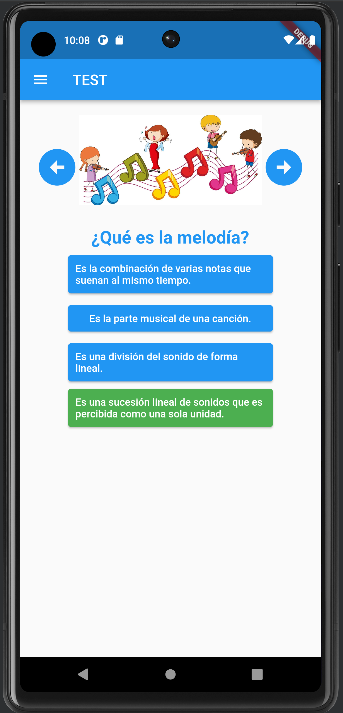
\includegraphics[width=0.4\textwidth]{imagenes/c7/selecunicab.png} }}%
  \qquad
  \subfloat[\centering Revisión de selección única fallida.]{{ 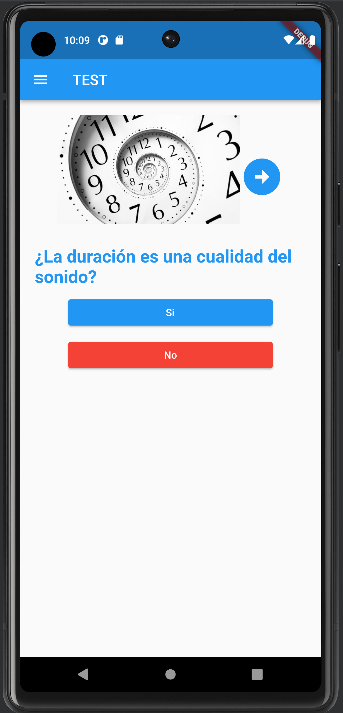
\includegraphics[width=0.4\textwidth]{imagenes/c7/selecunicab2.png} }}%
  \caption{Pantalla de la pregunta de selección única en revisión.}%
  \label{fig:revisar_unica}%
\end{figure}

\newpage

\subsubsection{Revisión de pregunta de selección múltiple}\mbox{}\\
\label{sec:pregunic1b}
\textit{Desarrollado en el Sprint 6}

\begin{figure}[H]%
  \centering
  \subfloat[\centering Selección múltiple acertada.]{{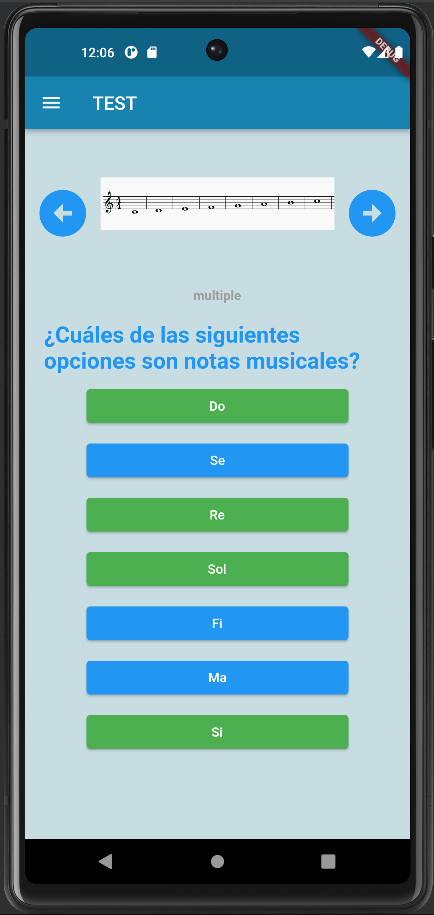
\includegraphics[width=0.45\textwidth]{imagenes/c7/selecmultib.png} }}%
  \qquad
  \subfloat[\centering Selección múltiple fallida.]{{ 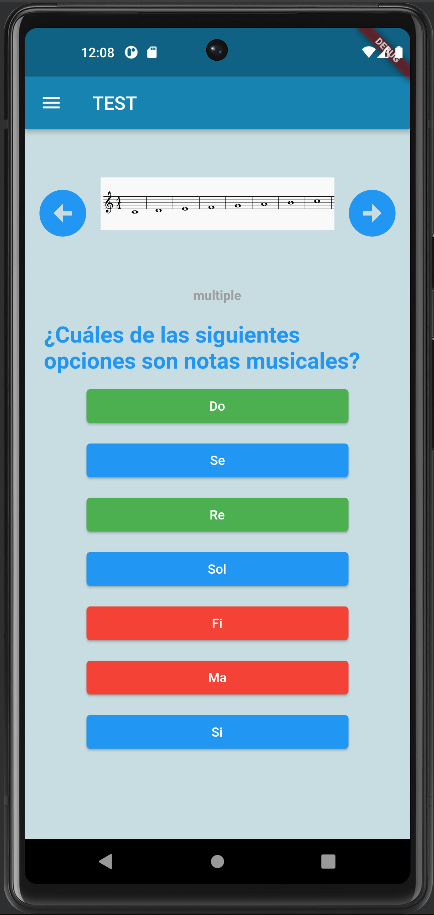
\includegraphics[width=0.45\textwidth]{imagenes/c7/selecmultib2.png} }}%
  \caption{Pantalla de la pregunta de selección múltiple en revisión.}%
  \label{fig:revisar_multiple}%
\end{figure}

\newpage

\subsubsection{Revisión de pregunta de entrada de texto}\mbox{}\\

\label{sec:pregunic1b}
\textit{Desarrollado en el Sprint 6}
\begin{figure}[H]%
  \centering
  \subfloat[\centering Revisión de entrada de texto acertada.]{{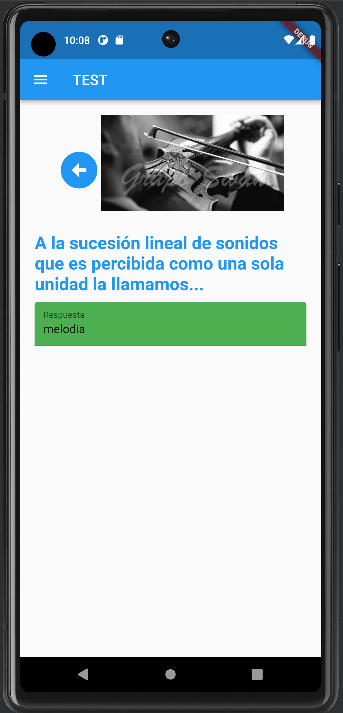
\includegraphics[width=0.45\textwidth]{imagenes/c7/entradatextob.png} }}%
  \qquad
  \subfloat[\centering Revisión de entrada de texto fallida.]{{ 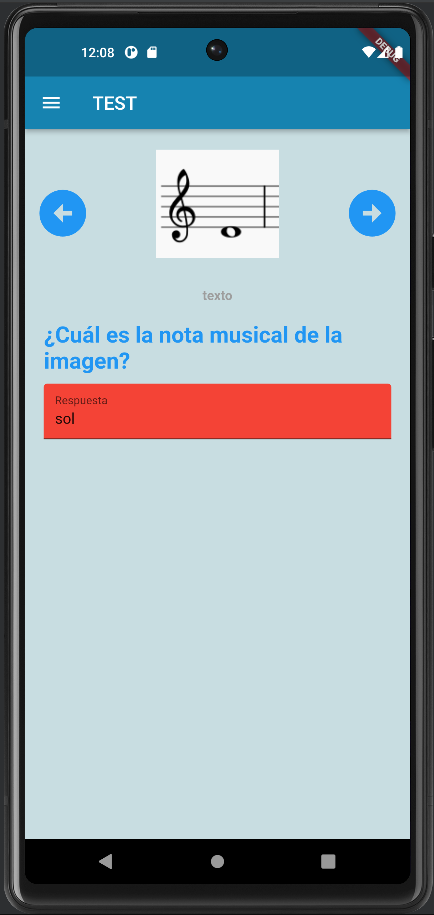
\includegraphics[width=0.45\textwidth]{imagenes/c7/entradatextob2.png} }}%
  \caption{Pantalla de la pregunta de entrada de texto en revisión.}%
  \label{fig:example}%
\end{figure}

\newpage

\subsubsection{Revisión de pregunta de entrada de micrófono}\mbox{}\\

\label{sec:pregunic1b}
\textit{Desarrollado en el Sprint 7}
\begin{figure}[H]%
  \centering
  \subfloat[\centering Revisión de entrada de micrófono acertada.]{{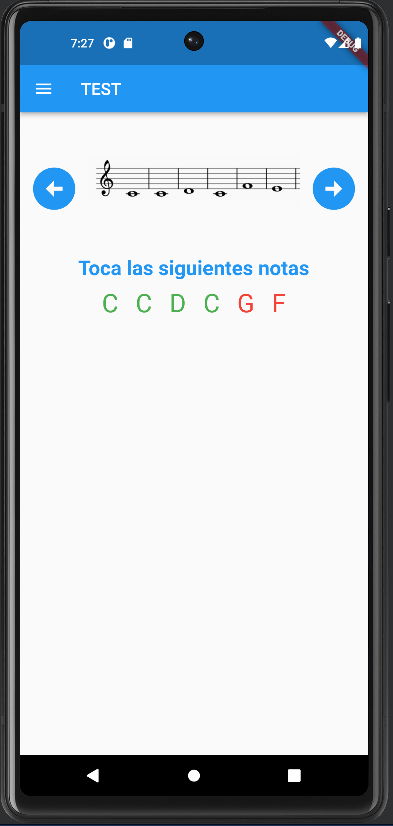
\includegraphics[width=0.45\textwidth]{imagenes/c7/entradamicrofonob.png} }}%
  \qquad
  \subfloat[\centering Revisión de entrada de micrófono fallida.]{{ 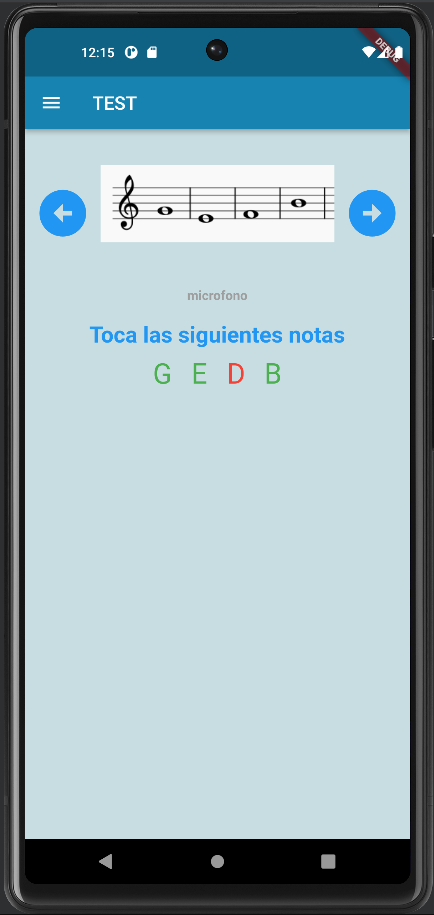
\includegraphics[width=0.45\textwidth]{imagenes/c7/entradamicrofonob2.png} }}%
  \caption{Pantalla de la pregunta de entrada de micrófono en revisión.}%
  \label{fig:example}%
\end{figure}

\newpage

\subsection{Historial de tests}
\textit{Desarrollado en el Sprint 6}
\label{sec:historial}

\paragraph*{Vista}
\label{sec:vista}
La vista de esta pantalla consiste en un distribuidor de columnas (Column) que contiene una lista de tests (ListView) verticalmente. 

\begin{figure}[H]
  \centering
  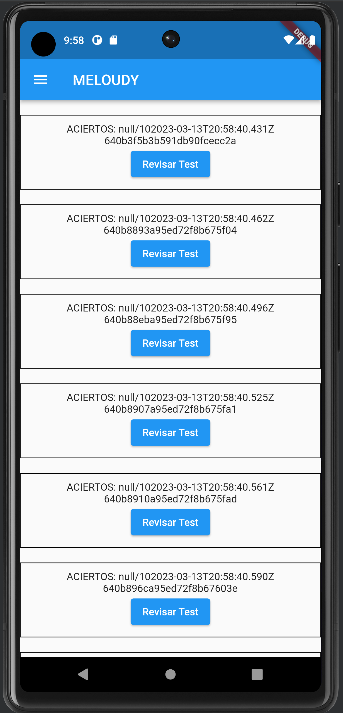
\includegraphics[width=0.44\textwidth]{imagenes/c7/historialtest.png}
  \caption{Pantalla de dashboard del profesor con las opciones de gestión disponibles para el administrador.}
  \label{fig:login}
\end{figure}


\subsection{Ver Mi Perfil}
\textit{Desarrollado en el Sprint 10}
\label{sec:miperfil}

\paragraph*{Vista}
\label{sec:vista}
Se ha utilizado un distribuidor de columnas (Column) que contienen los datos de los usuarios.
En la parte superior de la pantalla se muestra la foto de perfil del usuario, y debajo de la foto se muestra el nombre, 
el apellido, el nombre de usuario (username), el correo electrónico y el rol.


\begin{figure}[H]
  \centering
  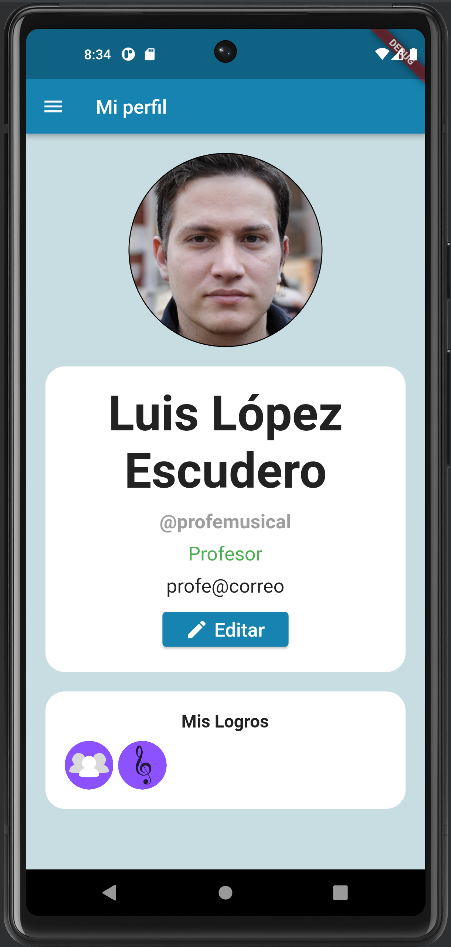
\includegraphics[width=0.44\textwidth]{imagenes/c7/miperfil.png}
  \caption{Pantalla del perfil del usuario.}
  \label{fig:login}
\end{figure}


\paragraph*{Lógica}
\label{sec:logica}
En primer lugar, cuando se accede al perfil se obtienen los datos del usuario
 mediante el método fetchAndSetUser de un nuevo Provider llamado UsuarioPerfil. Este método
manda una petición \textit{GET} a la ruta \textit{(/api/user/get-user/\{id\})}. Una vez obtenidos los datos del usuario mediante el provider UsuarioPerfil, estos se muestran en la vista. 


\subsection{Ver logro} 

\textit{Desarrollado en el Sprint 11}

Los usuarios podrán ver de forma detallada cada logro que hayan conseguido. Para ello, se ha desarrollado una pantalla que muestra la información de un único logro 
(imagen, título y descripción). A esta pantalla se accederá cuando el usuario pinche en uno de los logros dentro de su perfil.
\paragraph*{Vista}
Esta pantalla consta de un distribuidor de columnas (Column) de contenedores que contienen la información a mostrar. En la siguiente imagen se puede ver la pantalla de un logro: 

\begin{figure}[H]
  \centering
  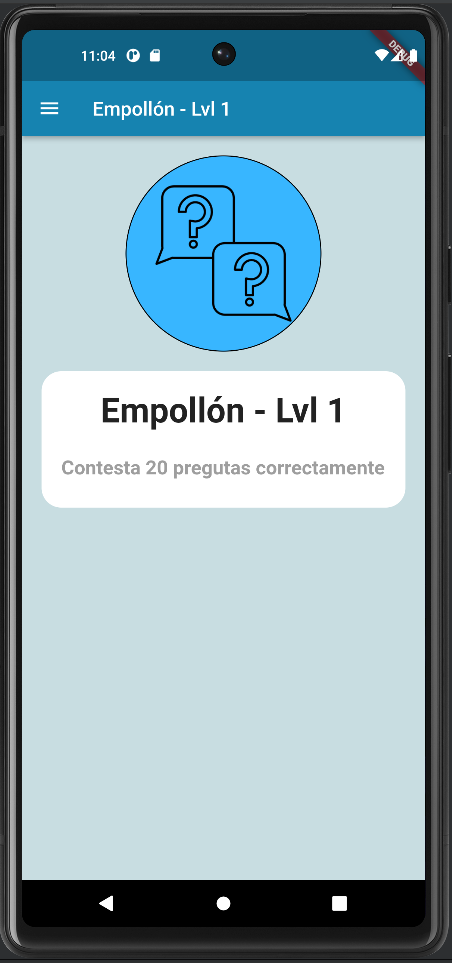
\includegraphics[width=0.38\textwidth]{imagenes/c7/verlogro.png}
  \caption{Pantalla de visualización de logro asignado.} 
  \label{fig:ver_logro}
\end{figure}

\paragraph*{Lógica}
Para cargar la información del logro no ha hecho falta llamar al provider pues la información del logro se encuentra en el provider UsuarioPerfil.
Por tanto, solo ha hecho falta obtener dichos datos y cargarlos en la nueva vista.

\subsection{Mis logros} 

\textit{Desarrollado en el Sprint 11}

Los usuarios podrán ver una lista de todos los logros que hayan conseguido. Hay que tener en cuenta que en el perfil del usuario solo se muestran algunos. 
A esta lista se accederá cuando el usuario pulse el botón "Más" de la sección de logros del perfil.
\paragraph*{Vista}
La información visual de esta funcionalidad consiste en un distribuidor de columnas (Column) de contenedores que contienen la información a mostrar de cada logro. 
Cada una de las filas contiene un distribuidor de filas (Row) que se encargará de visualizar a la izquierda la imagen de perfil y
 a la derecha la información de texto (esta última información a su vez está dentro de otro widget Column). 
 En la siguiente imagen se puede ver la pantalla de los logros del usuario:: 


\begin{figure}[H]
  \centering
  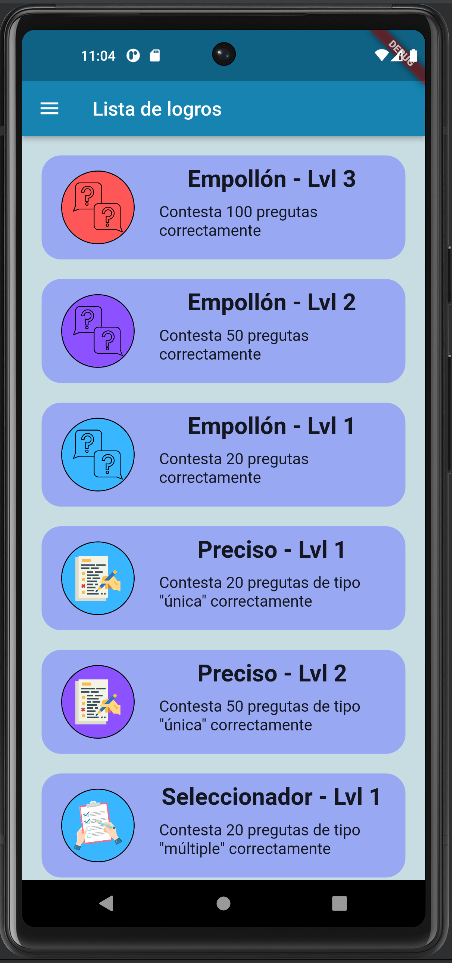
\includegraphics[width=0.38\textwidth]{imagenes/c7/listalogrosperfil.png}
  \caption{Pantalla de visualización de la lista de logros asignados.} 
  \label{fig:ver_logros_perfil}
\end{figure}



\paragraph*{Lógica}
Para cargar la lista de logros no ha hecho falta llamar al provider pues los datos de los logros se encuentran en el provider UsuarioPerfil.
Por tanto, solo ha hecho falta obtener dichos datos y cargarlos en la nueva vista.

\newpage

\section{Funcionalidad de gestión de la aplicación}
A continuación presentamos las funcionalidades de gestión de la aplicación. 
El profesor podrá gestionar las lecciones y las preguntas de la aplicación. 
Por otro lado, el administrador podrá gestionar, además de las lecciones y las preguntas, los usuarios y los logros de la aplicación.

\subsection{Dashboard}

\textit{Desarrollado en el Sprint 5}
\label{sec:dashboard}

Un dashboard es una interfaz de usuario que muestra información de forma resumida y que permite al usuario acceder a las diferentes funcionalidades de la aplicación.
 En este caso, el dashboard del profesor muestra las opciones de gestión de lecciones y preguntas.


\begin{figure}[H]%
  \centering
  \subfloat[\centering Pantalla de dashboard con las opciones de gestión disponibles para el administrador.]{{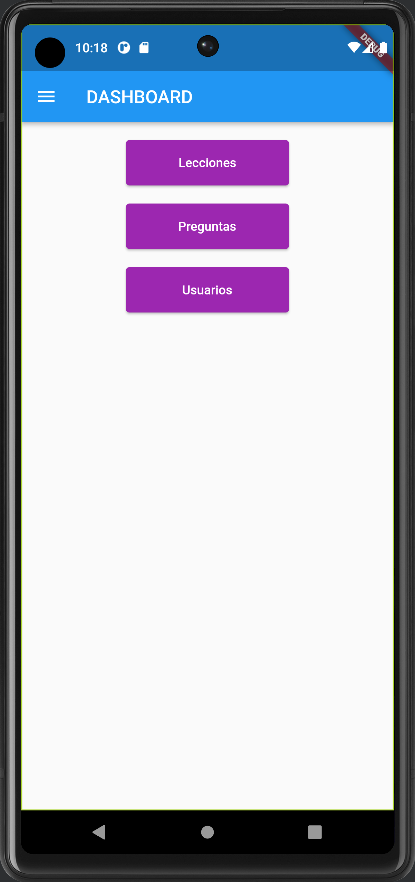
\includegraphics[width=0.35\textwidth]{imagenes/c7/dashboard.png} }}%
  \qquad
  \subfloat[\centering Composición de la pantalla de dashboard.]{{ 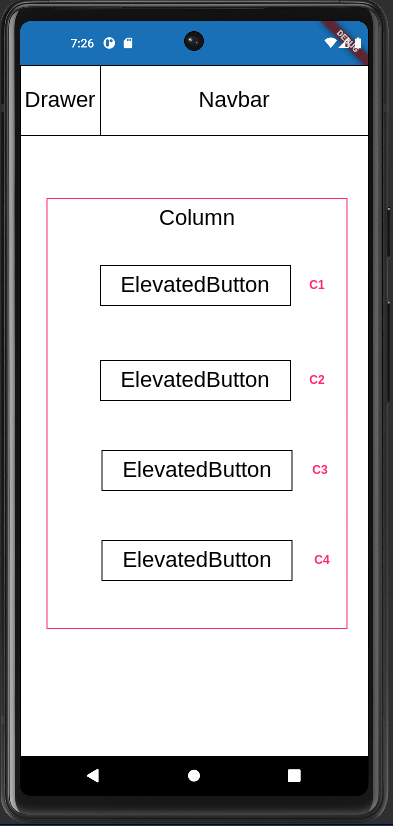
\includegraphics[width=0.35\textwidth]{imagenes/c7/dashboardcompo.png} }}%
  \caption{Vista del dashboard}%
  \label{fig:dashboard}%
\end{figure}

\paragraph*{Vista}
Se ha implementado una pantalla de dashboard para la gestión de la aplicación.
En esta pantalla, se muestran las opciones de gestión disponibles para la persona que utiliza la aplicación en función de su rol mediante una columna de ElevatedButton.
 En la figura \ref*{fig:dashboard} imagen se puede ver la pantalla de dashboard.




\subsection{Lista de lecciones} 
\textit{Desarrollado en el Sprint 5}

\paragraph*{Vista}
La lista de lecciones del profesor es muy similar a la del usuario. Las diferencias, aparte de los estilos, son los botones de tipo ElevatedButton
 que se han añadido para la gestión de las lecciones y que permiten al profesor crear, modificar y eliminar lecciones.
  En la siguiente imagen se puede ver la pantalla de lista de lecciones del profesor:

\begin{figure}[H]%
  \centering
  \subfloat[\centering Pantalla de lista de lecciones del profesor para la gestión de estas.]{{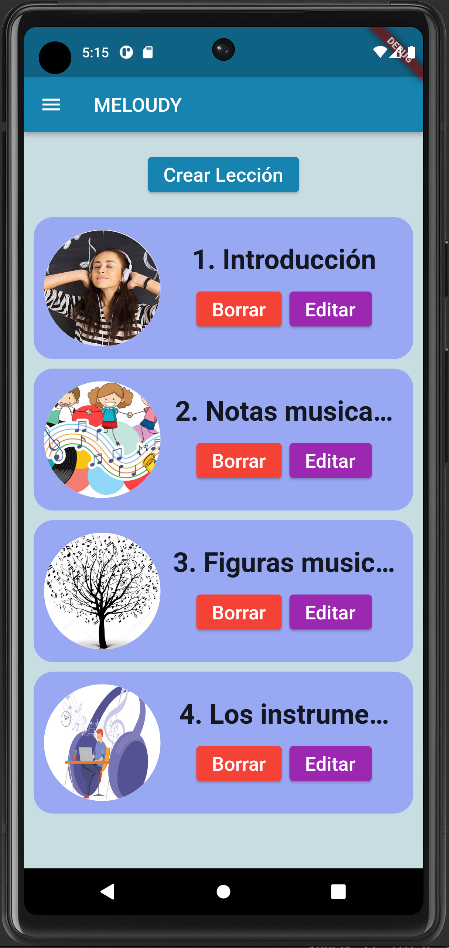
\includegraphics[width=0.45\textwidth]{imagenes/c7/listalecciones.png} }}%
  \qquad
  \subfloat[\centering Composición de la pantalla de la lista de lecciones.]{{ 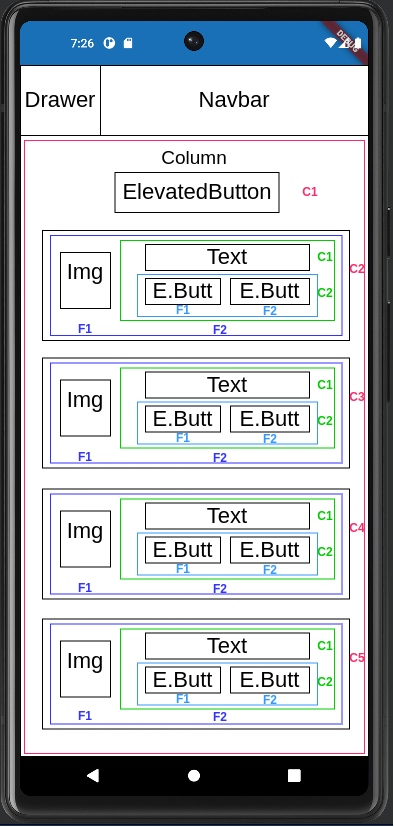
\includegraphics[width=0.45\textwidth]{imagenes/c7/leccionesprofe.png} }}%
  \caption{Vista de la lista de las lecciones.}%
  \label{fig:listalecciones}%
\end{figure}

\newpage

\subsection{Borrar lección} 

\textit{Desarrollado en el Sprint 8}
El profesor podrá borrar una lección de la lista de lecciones al pulsar el icono de la papelera mostrado en la vista del apartado anterior. 
Una vez pulsado, se mostrará un diálogo de confirmación para que el profesor confirme que desea borrar la lección.

\paragraph*{Vista}
La pantalla del borrado de lecciones utiliza el widget \textit{AlertDialog}, que posee
un título, un texto descriptivo y dos botones: uno para cancelar el borrado y otro para confirmarlo.
En la siguiente imagen se puede ver la pantalla de borrado de lecciones:


\begin{figure}[H]
  \centering
  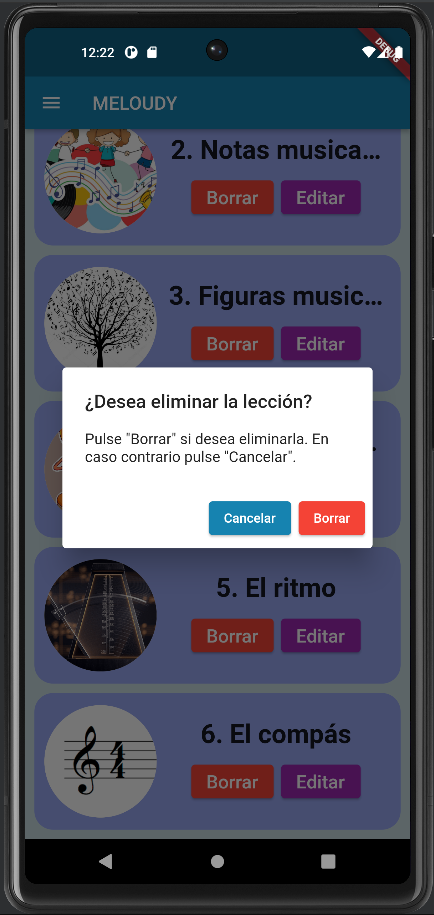
\includegraphics[width=0.5\textwidth]{imagenes/c7/borrarleccion.png}
  \caption{Pantalla del borrado de una lección.} 
  \label{fig:borradoleccion}
\end{figure}

\paragraph*{Lógica}
Una vez el botón de \textit{Confirmar} es pulsado, se muestra un diálogo de confirmación para que el profesor confirme que desea borrar la lección.
Este borrado se realiza llamando a la función borrarLeccion() del provider \textit{Lecciones}. 
En dicha función se borrará la lección de la lista del provider y se actualizará la base de datos enviando
una petición DELETE a la API con el id de la lección a borrar. La ruta de la petición es \textit{DELETE /api/lesson/delete-lesson}. 
La API devolverá un código de estado 200 si la operación se ha realizado correctamente y se actualizará la lista de lecciones del provider. 
En caso contrario, se mostrará un mensaje de error.


\subsection{Crear lección} 

\textit{Desarrollado en el Sprint 8}

Los profesores podrán crear lecciones para que los usuarios puedan estudiarlas. Para ello, se ha implementado una pantalla de creación de lecciones 
que permite al profesor añadir títulos, textos explicativos y contenido multimedia a la lección. Una vez creada, la lección se añadirá a la lista de lecciones del profesor.


\paragraph*{Vista}
La vista de esta pantalla consiste en un formulario de creación de lecciones. Este formulario consta de:
\begin{itemize}
  \item Un campo de texto para el título de la lección.
  \item Un botón para subir la imagen de la lección.
  \item Un número variable de campos de texto para los títulos.
  \item Un número variable de campos de texto para los textos explicativos.
  \item Un número variable de botones (\textit{ElevatedButton}) para las imágenes.
  \item Un número variable de campos de texto para los vídeos.
\end{itemize}

Todo esto está distribuido mediante el widget que organiza los elementos de forma vertical llamado \textit{Column}. 
En la parte inferior de la pantalla, se encuentran varios iconos organizados en una fila, que permiten incorporar nuevas widgets al contenido de la lección
ya que pulsando en uno de estos iconos, se añade un nuevo widget a la lista.

En las siguientes imágenes se puede ver la pantalla de creación de lecciones:

\begin{figure}[H]%
  \centering
  \subfloat[\centering Creación de lección vacía \#1.]{{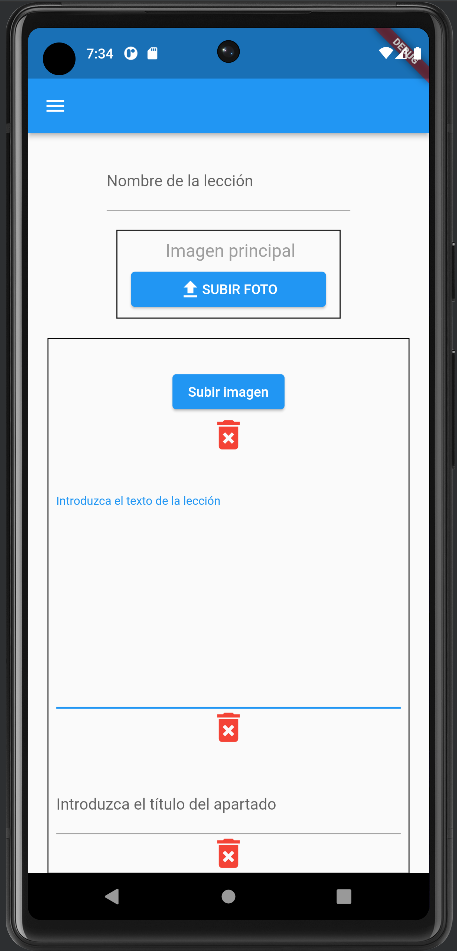
\includegraphics[width=0.44\textwidth]{imagenes/c7/crearleccion1.png} }}%
  \qquad
  \subfloat[\centering Creación de lección vacía \#2.]{{ 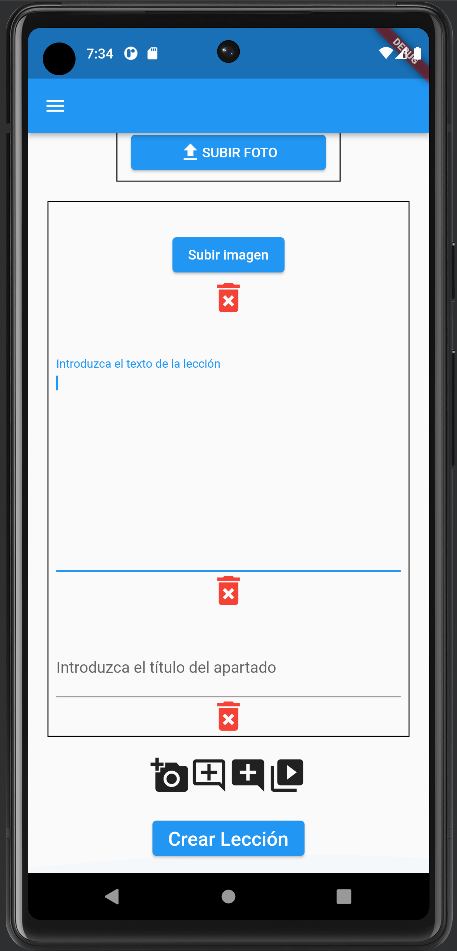
\includegraphics[width=0.44\textwidth]{imagenes/c7/crearleccion2.png} }}%
  \caption{Pantalla de la creación de lecciones sin datos introducidos.}%
  \label{fig:creacionleccionvacia}%
\end{figure}


\begin{figure}[H]%
  \centering
  \subfloat[\centering Creación de lección rellena \#1.]{{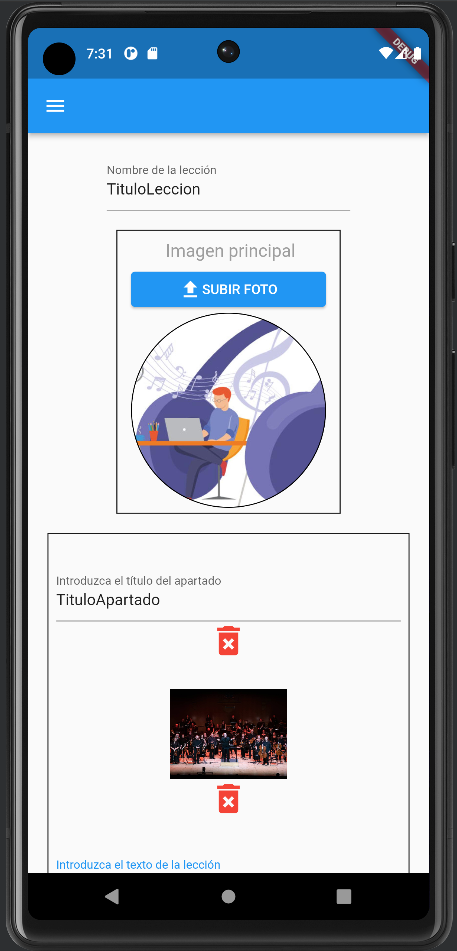
\includegraphics[width=0.45\textwidth]{imagenes/c7/crearleccion1b.png} }}%
  \qquad
  \subfloat[\centering Creación de lección rellena \#2.]{{ 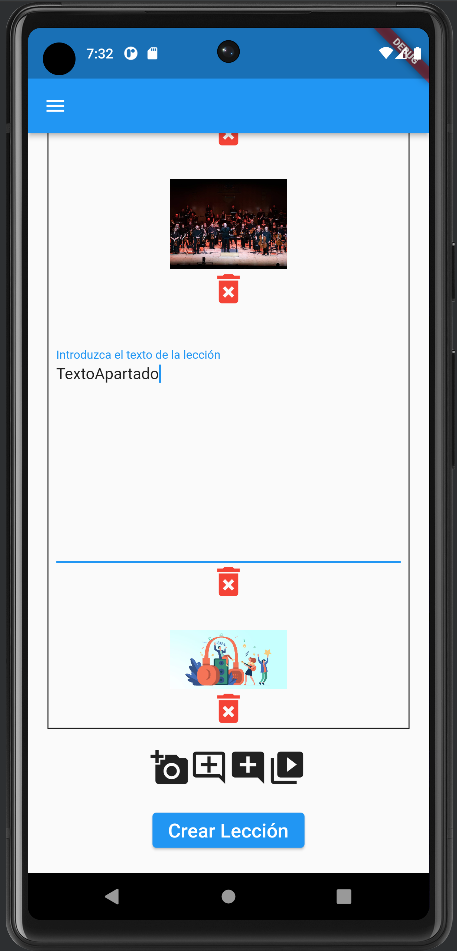
\includegraphics[width=0.45\textwidth]{imagenes/c7/crearleccion2b.png} }}%
  \caption{Pantalla de la creación de lecciones con datos introducidos. }%
  \label{fig:creacionleccionrellena}%
\end{figure}


\paragraph*{Lógica}
La funcionalidad de crear lección ha necesitado desarrollar varias utilidades debido a su complejidad. 
La primera de ellas es la de añadir campos de texto a la pantalla de creación de lecciones. 
Para ello, se han creado varios widgets que contienen un campo de texto y un botón para eliminar dicho campo. 
Estos widgets se han llamado \textit{SubirTexto}, \textit{SubirTitulo} y \textit{SubirVideo} y se añaden de forma dinámica a un vector ubicado 
en la pantalla de creación de lecciones al pulsar el botón correspondiente.

Para subir una imagen se ha hecho uso de la biblioteca \textit{image\_picker}, que permite al usuario seleccionar una imagen de su galería y
devuelve la ruta de la imagen seleccionada. Una vez tenemos el archivo de la imagen, se manda una petición de tipo multipart con la imagen a la API para que la suba al servidor.
El almacenamiento de la imagen utiliza la funcionalidad proporcionada por el paquete de NodeJS llamado \textit{multer} ~\cite{multerpackage}. 
Este paquete permite la subida de archivos al servidor y la creación de carpetas para almacenar dichos archivos.
La ruta de la petición es \textit{POST /api/lesson/upload-image}. La API devolverá un código de estado 200 si la operación se ha realizado correctamente. 
En caso contrario, se mostrará un mensaje de error.

El profesor también podrá eliminar widgets de la pantalla de creación de lecciones.
 Para ello, se ha implementado un botón en cada widget que permite al profesor eliminar dicho widget. Al pulsar este botón, se llama al método borrar(). 
 En este se elimina el widget de la lista y se actualiza la pantalla de creación de lecciones al ser un widget de tipo \textit{StatefulWidget}.

Una vez el usuario ha rellenado el formulario de creación de lecciones, se ha implementado un botón que permite al profesor guardar la lección. 
Al pulsar este botón, se envía una petición POST a la API con los datos de la lección. La ruta de la petición es \textit{POST /api/lesson/create-lesson}. 
La API devolverá un código de estado 200 si la operación se ha realizado correctamente y se actualizará la lista de lecciones del provider. 
En caso contrario, se mostrará un mensaje de error.


\subsection{Editar lección} 

\textit{Desarrollado en el Sprint 8}
Los profesores podrán editar la información y el contenido de las lecciones. Para ello, se ha implementado una pantalla de edición de lecciones 
que permite al profesor modificar el título, la imagen y todo el contenido.

\paragraph*{Vista}
La vista de esta pantalla es muy similar a la de la creación de lecciones. La diferencia es que los campos de texto continene la información de la lección que se está editando.

\begin{figure}[H]%
  \centering
  \subfloat[\centering Edición de lección \#1.]{{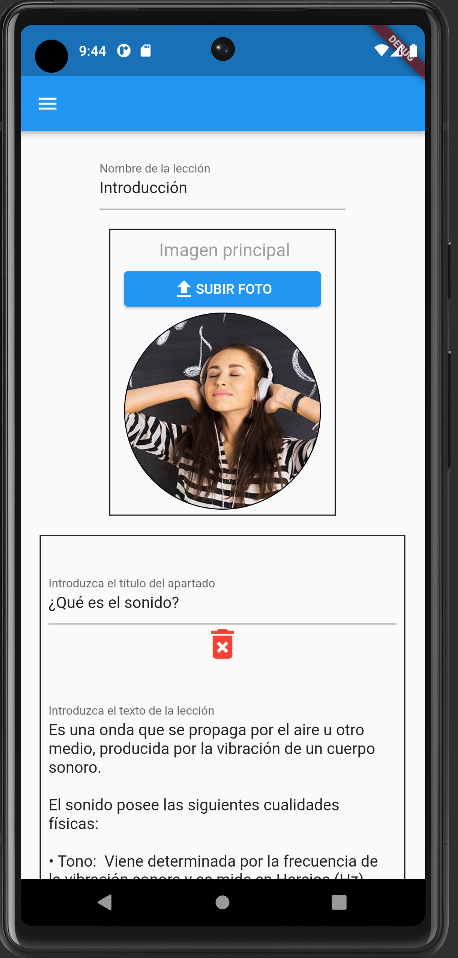
\includegraphics[width=0.4\textwidth]{imagenes/c7/editarleccion.png} }}%
  \qquad
  \subfloat[\centering Edición de lección \#2.]{{ 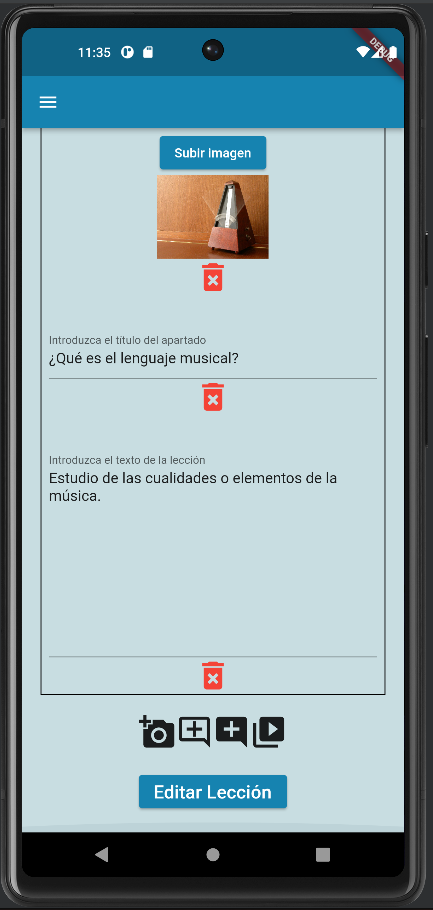
\includegraphics[width=0.4\textwidth]{imagenes/c7/editarleccion2.png} }}%
  \caption{Pantalla de la edición de lecciones existentes por parte del profesor.}%
  \label{fig:edicionleccion}%
\end{figure}


\paragraph*{Lógica}
En cuanto a la lógica, muchas de las funcionalidades de esta pantalla son iguales a las de la pantalla de creación de lecciones.

La única diferencia es que, al pulsar el botón de guardar, se envía una petición PUT a la API con los datos de la lección. 
La ruta de la petición es \textit{PUT /api/lesson/update-lesson}. La API devolverá un código de estado 200 si la operación se 
ha realizado correctamente y se actualizará la lista de lecciones del provider. En caso contrario, se mostrará un mensaje de error.

\newpage
\subsection{Lista de preguntas} 

\textit{Desarrollado en el Sprint 8}

\paragraph*{Vista}
La lista de preguntas contiene todas las preguntas existentes en el sistema. Se ha utilizado un distribuidor de columnas /textit{(Column)} para mostrar las preguntas verticalmente. 
Cada pregunta tiene un distribuidor de elementos horizontal /textit{(Row)} que contiene a la izquierda la imagen de la pregunta y 
a la derecha el texto de la cuestión, el tipo de pregunta y su identificador. Además de esto, cada pregunta tiene un icono de tipo Icon que permite al usuario modificar la pregunta.
\begin{figure}[H]
  \centering
  \includegraphics[width=0.4\textwidth]{imagenes/c7/listapreguntas.png}
  \caption{Pantalla de lista de preguntas del profesor para la gestión de estas.} 
  \label{fig:listapreguntas}
\end{figure}

\newpage
\subsection{Borrar pregunta} 

\textit{Desarrollado en el Sprint 9}

El profesor podrá borrar una pregunta de la lista al pulsar el icono de la papelera mostrado en la vista del apartado anterior.
 Una vez pulsado, se mostrará un diálogo de confirmación para que el profesor confirme que desea borrar la pregunta.

\paragraph*{Vista}
La pantalla del borrado de preguntas utiliza el widget \textit{AlertDialog}, que posee
un título, un texto descriptivo y dos botones: uno para cancelar el borrado y otro para confirmarlo.
En la siguiente imagen se puede ver la pantalla de borrado de preguntas:


\begin{figure}[H]
  \centering
  \includegraphics[width=0.5\textwidth]{imagenes/c7/borrarpregunta.png}
  \caption{Pantalla del borrado de una pregunta.} 
  \label{fig:borradopregunta}
\end{figure}

\paragraph*{Lógica}
Una vez el botón de \textit{Confirmar} es pulsado, se muestra un diálogo de confirmación para que el profesor confirme que desea borrar la pregunta.
Este borrado se realiza llamando a la función borrarPregunta() del provider \textit{PreguntasProfesor}. En dicha función se borrará la pregunta 
de la lista del provider y se actualizará la base de datos enviando una petición DELETE a la API con el id de la pregunta a borrar. 
La ruta de la petición es \textit{DELETE /api/question/delete-question}.La API devolverá un código de estado 200 si 
la operación se ha realizado correctamente y se actualizará la lista de preguntas del provider. En caso contrario, se mostrará un mensaje de error.


\subsection{Crear Pregunta} 

\textit{Desarrollado en el Sprint 9}

Los profesores podrán crear preguntas para que los usuarios puedan contestarlas en los tests. 
Para ello, se ha implementado una pantalla de creación de preguntas que permite al profesor elegir el tipo de pregunta y modificar 
toda la información relacionada con esta (imagen, opciones, respuestas correctas, etc). Una vez creada, la lección se añadirá a la lista de lecciones del profesor.



\paragraph*{Vista}
La vista de esta pantalla consiste en un formulario de creación de preguntas. Este formulario consta de:
\begin{itemize}
  \item Un desplegable para elegir el tipo de pregunta (entre \textit{única, múltiple, micrófono y texto}).
  \item Un botón para subir la imagen de la pregunta.
  \item Un desplegable para elegir la lección a la que pertenece la pregunta.
  \item Un campo de texto para el enunciado/cuestión de la pregunta.
  \item Si es una pregunta de tipo 'única' o 'múltiple', un número variable de campos de texto para las opciones de la pregunta.
  \item Si es una pregunta de tipo 'texto', un campo de texto para la respuesta correcta.
  \item Si es una pregunta de tipo 'micrófono', un número variable de desplegables para elegir las notas musicales correctas.
\end{itemize}


\newpage
Todo esto está distribuido mediante el widget que organiza los elementos de forma vertical llamado \textit{Column}. 
Dentro de este, se encuentran los widgets del formulario, que serán desde widgets de desplegables (\textit{DropdownButton}) 
hasta widgets de campos de texto (\textit{TextField}), pasando por casillas de verificación (\textit{Checkbox}).
En las preguntas de tipo 'única', 'múltiple' y 'micrófono', en la parte inferior de la pantalla se encuentra un icono que permite al profesor añadir más opciones a la pregunta.

En las siguientes imágenes se puede ver la pantalla de creación de preguntas de todos los tipos con los campos de texto vacíos y rellenos.
\begin{figure}[H]
  \centering
  \includegraphics[width=0.45\textwidth]{imagenes/c7/crearpreguntaunica1.png}
  \caption{Pantalla de creación de pregunta de tipo 'única' vacía. La pregunta de tipo múltiple y de tipo micrófono son iguales.} 
  \label{fig:crearpreguntaunica}
\end{figure}


\begin{figure}[H]%
  \centering
  \subfloat[\centering Creación de pregunta 'única' rellena \#1.]{{\includegraphics[width=0.30\textwidth]{imagenes/c7/crearpreguntaunica2.png} }}%
  \qquad
  \subfloat[\centering Creación de pregunta 'única' rellena \#2.]{{ \includegraphics[width=0.30\textwidth]{imagenes/c7/crearpreguntaunica3.png} }}%
  \caption{Pantalla de creación de pregunta de tipo 'única' con datos introducidos.}%
  \label{fig:crearpreguntaunica}%
\end{figure}


\begin{figure}[H]%
  \centering
  \subfloat[\centering Creación de pregunta 'múltiple' rellena \#1.]{{\includegraphics[width=0.30\textwidth]{imagenes/c7/crearpreguntamultiple2.png} }}%
  \qquad
  \subfloat[\centering Creación de pregunta 'múltiple' rellena \#2.]{{ \includegraphics[width=0.30\textwidth]{imagenes/c7/crearpreguntamultiple3.png} }}%
  \caption{Pantalla de creación de pregunta de tipo 'múltiple' con datos introducidos.}%
  \label{fig:crearpreguntamultiple}%
\end{figure}



\begin{figure}[H]%
  \centering
  \subfloat[\centering Creación de pregunta 'micrófono' rellena \#1.]{{\includegraphics[width=0.30\textwidth]{imagenes/c7/crearpreguntamicrofono1.png} }}%
  \qquad
  \subfloat[\centering Creación de pregunta 'micrófono' rellena \#2.]{{ \includegraphics[width=0.30\textwidth]{imagenes/c7/crearpreguntamicrofono2.png} }}%
  \caption{Pantalla de creación de pregunta de tipo 'micrófono' con datos introducidos.}%
  \label{fig:crearpreguntamicrofono}%
\end{figure}

\begin{figure}[H]%
  \centering
  \subfloat[\centering Creación de pregunta 'texto' vacía.]{{\includegraphics[width=0.30\textwidth]{imagenes/c7/crearpreguntatexto1.png} }}%
  \qquad
  \subfloat[\centering Creación de pregunta 'texto' rellena.]{{ \includegraphics[width=0.30\textwidth]{imagenes/c7/crearpreguntatexto2.png} }}%
  \caption{Pantalla de creación de pregunta de tipo 'texto'.}%
  \label{fig:crearpreguntatexto}%
\end{figure}



\paragraph*{Lógica}
La funcionalidad de crear preguntas se ha implementado utilizando el Provider de preguntas anteriormente mencionado. De esta forma
se ha podido comunicar varias pantallas entre sí y compartir datos entre ellas. 

Para empezar, se ha creado un nuevo widget llamado \textit{SubirOpcion}, que actua de forma muy parecida a los widgets mencionados 
en la creación de lecciones (SubirImagen, SubirTitulo, SubirTexto...). Este widget se encargará de encapsular toda la vista y la lógica relacionada con una opción concreta.
Además he visto necesaria la creación de un nuevo Provider para las opciones de las preguntas. Este Provider contiene un vector de opciones y un vector de respuestas correctas.
El vector de opciones contiene los textos de las opciones de la pregunta y el vector de respuestas correctas contiene los índices de las opciones correctas.
Estos dos vectores se actualizan cada vez que el profesor añade o elimina una opción de la pregunta. 
De esta forma, la comunicación entre la pantalla y la clase "SubirOpcion" ha sido más sencilla tanto para borrar una opción como para desmarcar una opción cuando se marca otra distinta.
El widget de SubirOpcion se añade de forma dinámica a un vector de widgets ubicado en la pantalla de creación de preguntas al pulsar el botón correspondiente.


Para subir una imagen se ha hecho uso de nuevo de la biblioteca \textit{image\_picker}, que detallé en la funcionalidad de crear lecciones.
El profesor podrá eliminar widgets mediante el botón apropiado en cada uno de ellos. Dicho botón llama al método borrar() y 
éste elimina el widget de la listas y actualiza la pantalla de creación de preguntas.

El botón de guardar la lección envía los datos de las preguntas al servidor mediante una petición POST a la ruta /api/question/create-question.
 La API devolverá un código de estado 200 si la operación se ha realizado correctamente y se actualizará la lista de preguntas del provider. 
 En caso contrario, se mostrará un mensaje de error.

\newpage

\subsection{Editar Pregunta} 

\textit{Desarrollado en el Sprint 9}
Los profesores podrán editar la información y el contenido de las preguntas. Para ello, se ha implementado una pantalla de edición 
de preguntas que permite al profesor modificar la cuestión, la imagen y todos los demás datos.

\paragraph*{Vista}
La vista de esta pantalla es muy similar a la de la creación de las preguntas. La diferencia es que los widgets disponen de la información de la pregunta que se está editando.

\begin{figure}[H]%
  \centering
  \subfloat[\centering Edición de pregunta única \#1.]{{\includegraphics[width=0.45\textwidth]{imagenes/c7/editarpreguntaunica1.png} }}%
  \qquad
  \subfloat[\centering Edición de pregunta única\#2.]{{ \includegraphics[width=0.45\textwidth]{imagenes/c7/editarpreguntaunica2.png} }}%
  \caption{Pantalla de edición de pregunta de tipo 'única'.}%
  \label{fig:edición_pregunta_unica}%
\end{figure}



\begin{figure}[H]%
  \centering
  \subfloat[\centering Edición de pregunta múltiple\#1.]{{\includegraphics[width=0.30\textwidth]{imagenes/c7/editarpreguntamultiple1.png} }}%
  \qquad
  \subfloat[\centering Edición de pregunta múltiple\#2.]{{ \includegraphics[width=0.30\textwidth]{imagenes/c7/editarpreguntamultiple2.png} }}%
  \caption{Pantalla de edición de pregunta de tipo 'múltiple'.}%
  \label{fig:edición_pregunta_multiple}%
\end{figure}


\begin{figure}[H]
  \centering
  \includegraphics[width=0.32\textwidth]{imagenes/c7/editarpreguntamicrofono.png}
  \caption{Pantalla de edición de pregunta de tipo 'micrófono'.} 
  \label{fig:edición_pregunta_microfono}
\end{figure}

\begin{figure}[H]
  \centering
  \includegraphics[width=0.32\textwidth]{imagenes/c7/editarpreguntatexto.png}
  \caption{Pantalla de edición de pregunta de tipo 'texto'.} 
  \label{fig:edición_pregunta_tecto}
\end{figure}


\paragraph*{Lógica}
En cuanto a la lógica, muchas de las funcionalidades de esta pantalla son iguales a las de la pantalla de creación de preguntas.
Entre las diferencias notamos que al entrar se deben inicializar los valores de cada uno de los campos con aquellos obtenidos de
 la base de datos y que, al pulsar el botón de guardar, se envía una petición PUT a la API con los datos de la pregunta. 
 La ruta de la petición es \textit{PUT /api/question/update-question}. La API devolverá un código de estado 200 si 
 la operación se ha realizado correctamente y se actualizará la lista de preguntas del provider. En caso contrario, se mostrará un mensaje de error.


\newpage
\subsection{Lista de usuarios} 

\textit{Desarrollado en el Sprint 9}

\paragraph*{Vista}
La lista de usuarios contiene todos los usuarios registrados en el sistema. Se ha utilizado un distribuidor de columnas /textit{(Column)} para mostrar los usuarios de forma vertical. 
Cada usuario tiene un distribuidor de elementos horizontal /textit{(Row)} que contiene a la izquierda la foto del usuario y 
a la derecha su nombre en negrita y el correo en un color grisáceo. 

\begin{figure}[H]
  \centering
  \includegraphics[width=0.4\textwidth]{imagenes/c7/listausuarios.png}
  \caption{Pantalla de lista de usuarios del administrador para la gestión de estos.} 
  \label{fig:listausuarios}
\end{figure}

\subsection{Borrar usuario} 

\textit{Desarrollado en el Sprint 10}

El administrador podrá borrar un usuario de la lista al pulsar en el botón de "Borrar" mostrado en la Figura \ref{fig:listausuarios}.
Una vez pulsado, se mostrará un diálogo para que el administrador confirme que desea borrar el usuario.

\paragraph*{Vista}
La pantalla del borrado de usuarios utiliza el widget \textit{AlertDialog}, que posee
un título, un texto descriptivo y dos botones: uno para cancelar el borrado y otro para confirmarlo.
En la siguiente imagen se puede ver la pantalla de borrado de usuarios:


\begin{figure}[H]
  \centering
  \includegraphics[width=0.5\textwidth]{imagenes/c7/borrarusuario.png}
  \caption{Pantalla de borrado de un usuario.} 
  \label{fig:borradousuario}
\end{figure}

\paragraph*{Lógica}
Una vez pulsado el botón de \textit{Borrar}, se muestra un diálogo para que el administrador confirme que desea borrar el usuario. Este borrado se hará
 llamando a la función borrarUsuario() del provider \textit{Usuarios}. En dicha función se borrará el usuario de la lista del provider 
y se actualizará la base de datos enviando una petición DELETE a la API con el id del usuario a borrar. La ruta de la petición es \textit{DELETE /api/user/delete-user}. 
La API devolverá un código de estado 200 si la operación se ha realizado correctamente y se actualizará la lista de usuarios del provider. En caso contrario, 
se mostrará un mensaje de error.

\subsection{Crear usuario} 

\textit{Desarrollado en el Sprint 10}

Los administradores podrán crear usuarios en el sistema. Para ello, se ha implementado una pantalla de creación de usuarios que permite 
introducir los datos del usuario: nombre, el correo, la contraseña, la foto... Una vez creado, el usuario se añadirá a la lista de usuarios del profesor.


\paragraph*{Vista}
La vista de esta pantalla consiste en un formulario de creación de usuarios. Este formulario consta de:
\begin{itemize}
  \item Un botón para subir la imagen del usuario.
  \item Un desplegable para elegir el rol del usuario.
  \item Campos de texto para introducir el nombre, los apellidos, el nombre de usuario, el correo y la contraseña.
\end{itemize}


Todo esto está distribuido mediante el widget que organiza los elementos de forma vertical llamado \textit{Column}. 
Dentro de este, se encuentran los widgets del formulario, que serán tanto widgets de desplegables (\textit{DropdownButton}) como widgets de campos de texto (\textit{TextField}).

En las siguientes imágenes se puede ver la pantalla de creación de usuarios de todos los tipos con los campos de texto vacíos y rellenos.


\begin{figure}[H]%
  \centering
  \subfloat[\centering Creación de usuario vacía. \#1.]{{\includegraphics[width=0.32\textwidth]{imagenes/c7/crearusuario1.png} }}%
  \qquad
  \subfloat[\centering Creación de usuario rellena \#2.]{{ \includegraphics[width=0.32\textwidth]{imagenes/c7/crearusuario2.png} }}%
  \caption{Pantallas de creación de usuarios.}%
  \label{fig:creacionusuario}%
\end{figure}



\paragraph*{Lógica}
La funcionalidad de crear usuarios se ha implementado utilizando un nuevo método de creación de usuarios del Provider llamado usuarios. De esta forma
se ha podido comunicar varias pantallas entre sí y añadir el usuario creado a la lista de usuarios del administrador.


Para subir una imagen se ha hecho uso de nuevo de la biblioteca \textit{image\_picker}, que detallé en la funcionalidad de crear lecciones.

El botón de guardar el usuario envía los datos de los usuarios al servidor mediante una petición POST a la ruta /api/user/registro. 
La API devolverá un código de estado 200 si la operación se ha realizado correctamente y se actualizará la lista de usuarios del provider. 
En caso contrario, se mostrará un mensaje de error.

\newpage

\subsection{Editar usuario} 

\textit{Desarrollado en el Sprint 10}

Los administradores podrán editar la información de los usuarios. Para ello, se ha implementado una pantalla de edición de usuarios 
que permite al profesor modificar el nombre, los apellidos, la foto y todos los demás datos.

\paragraph*{Vista}
La vista de esta pantalla es muy similar a la de la creación de los usuarios. La diferencia es que los widgets disponen de la información del usuario que se está editando.

\begin{figure}[H]
  \centering
  \includegraphics[width=0.36\textwidth]{imagenes/c7/editarusuario.png}
  \caption{Pantalla de edición de usuario existente.} 
  \label{fig:edicion_usuario}
\end{figure}


\paragraph*{Lógica}
Los datos del usuario se inician con la información almacenada en la base de datos. Una vez confirmadas las modificaciones, 
se envía una petición PUT a la API con los datos actualizados del usuario a la ruta \textit{/api/user/update-user}. 
La API devolverá un código de estado 200 si la operación se ha realizado correctamente y se actualizará la lista de usuarios del provider. 
En caso contrario, se mostrará un mensaje de error.


\subsection{Lista de logros} 

\textit{Desarrollado en el Sprint 10}
\paragraph*{Vista}
La lista de logros contiene todos los logros creados en el sistema. Se ha utilizado un distribuidor de columnas /textit{(Column)} para mostrar los logros de forma vertical. 
Cada logro tiene un distribuidor de elementos horizontal /textit{(Row)} que contiene a la izquierda la imagen del logro y a la derecha el nombre en negrita. 

\begin{figure}[H]
  \centering
  \includegraphics[width=0.37\textwidth]{imagenes/c7/listalogros.png}
  \caption{Pantalla de lista de logros del administrador.} 
  \label{fig:listalogros}
\end{figure}


\subsection{Borrar logro} 

\textit{Desarrollado en el Sprint 10}
El administrador podrá borrar un logro de la lista al pulsar el botón \"Borrar\" mostrado en la vista de la figura \ref{fig:listalogros}. 
Una vez pulsado, se mostrará un diálogo de confirmación para que el administrador confirme que desea borrar el logro.

\newpage
\paragraph*{Vista}
La pantalla del borrado de logros utiliza el widget \textit{AlertDialog}, que posee
un título, un texto descriptivo y dos botones: uno para cancelar el borrado y otro para confirmarlo.
En la siguiente imagen se puede ver la pantalla de borrado de logros:


\begin{figure}[H]
  \centering
  \includegraphics[width=0.45\textwidth]{imagenes/c7/borrarlogro.png}
  \caption{Pantalla del borrado de un logro.} 
  \label{fig:borradologro}
\end{figure}

\paragraph*{Lógica}
Una vez pulsado el botón de \textit{Borrar}, se muestra un diálogo para que el administrador confirme que desea borrar el logro.
Este borrado se realiza llamando a la función borrarLogro() del provider \textit{Logros}. 
En dicha función se borrará el logro de la lista del provider y se actualizará la base de datos enviando
una petición \textit{DELETE} a la ruta \textit{/api/achievement/delete-achievement}. 
La API devolverá un código de estado 200 si la operación se ha realizado correctamente y se actualizará la lista de logros del provider. 
En caso contrario, se mostrará un mensaje de error.



\subsection{Crear logro} 

\textit{Desarrollado en el Sprint 10}

Los administradores podrán crear logros en el sistema. Para ello, se ha implementado una pantalla de creación de logros que permite introducir 
el nombre, la imagen, la descripción, el tipo y la condición del logro. Una vez creado, se añadirá a la lista de logros de la pantalla del administrador.


\paragraph*{Vista}
La vista de esta pantalla consiste en un formulario de creación de logros. Este formulario consta de:
\begin{itemize}
  \item Un botón para subir la imagen del logro.
  \item Un campo de texto para introducir el nombre del logro.
  \item Un campo de texto para introducir la descripción del logro.
  \item Un desplegable para elegir el tipo de logro (entre \textit{amigos, lección, lecciones, tests, preguntas, preguntasunica, preguntasmultiple, preguntasmicrofono y preguntastexto}).  
  \item Si el logro no es de tipo \'leccion\', un campo de texto para introducir la condición dependiente del tipo.
  \item Si el logro es de tipo \'leccion\', un desplegable para elegir la lección a la que pertenece el logro.
\end{itemize}

\begin{figure}[H]%
  \centering
  \subfloat[\centering Creación de logro vacío. \#1.]{{\includegraphics[width=0.35\textwidth]{imagenes/c7/crearlogro1.png} }}%
  \qquad
  \subfloat[\centering Creación de logro rellena \#2.]{{ \includegraphics[width=0.35\textwidth]{imagenes/c7/crearlogro2.png} }}%
  \caption{Pantallas de creación de logros.}%
  \label{fig:creacion_logros}%
\end{figure}

\newpage

Todo esto está distribuido mediante el widget que organiza los elementos de forma vertical llamado \textit{Column}.

En las imágenes anteriores se puede ver la pantalla de creación de logros con los campos de texto vacíos y rellenos.



\paragraph*{Lógica}
Se ha implementado utilizando un nuevo método de creación de logros del Provider llamado logros. De esta forma
se ha podido comunicar varias pantallas entre sí y añadir el logro creado a la lista de logros del administrador.


Para subir una imagen se ha hecho uso de nuevo de la biblioteca \textit{image\_picker}, que detallé en la funcionalidad de crear lecciones.

El botón de guardar el logro envía los datos de los logros al servidor mediante una petición POST a la ruta /api/achievement/create-achievement. 
La API devolverá un código de estado 200 si la operación se ha realizado correctamente y se actualizará la lista de logros del provider. 
En caso contrario, se mostrará un mensaje de error.


\subsection{Editar logro} 

\textit{Desarrollado en el Sprint 10}

Los administradores podrán editar la información de los logros. Para ello, se ha implementado una pantalla de edición de logros 
que permite al administrador modificar el nombre, la imagen, la descripción, el tipo y la condición del logro.

\paragraph*{Vista}
La vista de esta pantalla es muy similar a la de la creación de los logros. La diferencia es que los widgets disponen de la información del logro que se está editando.

\begin{figure}[H]
  \centering
  \includegraphics[width=0.38\textwidth]{imagenes/c7/editarlogro.png}
  \caption{Pantalla de edición de logro existente.} 
  \label{fig:edicion_logro}
\end{figure}


\paragraph*{Lógica}
Los datos del logro se inician con la información almacenada en la base de datos. Una vez confirmadas las modificaciones, 
se envía una petición PUT a la API con los datos actualizados del logro a la ruta \textit{/api/achievement/update-achievement}. 
La API devolverá un código de estado 200 si la operación se ha realizado correctamente y se actualizará la lista de logros del provider. 
En caso contrario, se mostrará un mensaje de error.

